\documentclass[11pt, twoside, pdftex]{article}

% This include all the settings that we should use for the document
\newcommand{\PDFTitle}{Debugging of VHDL Hardware Designs on Intel's DE-Series Boards}
\newcommand{\commonPath}{../../../Common}
\newcommand{\datePublished}{Mar 2022}

\newcommand{\versnum}{21.1} %version number quartus/AMP
\newcommand{\quartusname}{Quartus\textsuperscript{\textregistered} Prime}	
\newcommand{\textBar}{For \quartusname{} \versnum{}}
\newcommand{\thisyear}{2022 } %for copyright
\newcommand{\company}{FPGAcademy.org}
\newcommand{\longteamname}{FPGAcademy.org}
\newcommand{\teamname}{FPGAcademy}
\newcommand{\website}{FPGAcademy.org}

\newcommand{\productAcronym}{AMP}
\newcommand{\productNameShort}{Monitor Program}

\newcommand{\productNameMedTM}{Monitor Program}
\newcommand{\productNameMed}{Monitor Program}

%\newcommand{\headerLogoFilePath}[1]{#1/FPGAcademy.png}



\setlength\topmargin{-0.25in}
\setlength\headheight{0in}
\setlength\headsep{0.35in}
\setlength\textheight{8.5in}
\setlength\textwidth{7in}
\setlength\oddsidemargin{-0.25in}
\setlength\evensidemargin{-0.25in}
\setlength\parindent{0.25in}
\setlength\parskip{0in} 

\pdfpagewidth 8.5in
\pdfpageheight 11in

% listings is a package that supports encapsulating source code in LaTeX conveniently

\usepackage{listings}
% add support for graphics
\usepackage{graphicx}
\usepackage[usenames, dvipsnames]{color}

\def\expandparam\lstinputlisting[#1]#2{\edef\tmp{\noexpand\lstinputlisting[#1]{#2}}\tmp}

\widowpenalty 10000
\clubpenalty 10000

%%%%%%%%%%%%%%%%%%%% Source Code Formatting %%%%%%%%%%%%%%%%%%%%
\definecolor{globalCommentColour}{rgb}{0.588,0.588,0.588}

%%%%%%%%%%%%%%%%%%%%%%%%%%%%%%%%%%%%%%%%%%%%%%%%%%%%
% Defining a NiosII ASM highlighter for lstlisting
\lstdefinelanguage[NiosII]{Assembler} {
 	morekeywords={add, addi, and, andhi, andi, beq, bge, bgeu, bgt, bgtu, ble,  bleu, blt, bltu, bne, br, break,% 
 	bret, call, callr, cmpeq, cmpeqi, cmpge, cmpgei, cmpgeu, cmpgeui, cmpgt, cmpgti, cmpgtu, cmpgtui, cmple,%
 	cmplei, cmpleu, cmpleui, cmplt, cmplti, cmpltu, cmpltui, cmpne, cmpnei, custom, div, divu, eret, flushd,%
 	flushda, flushi, flushp, initd, initda, initi, jmp, jmpi, ldb, ldbio, ldbu, ldbuio, ldh, ldhio, ldhu, ldhuio,%
 	ldw, ldwio, mov, movhi, movi, movia, movui, mul, muli, mulxss, mulxsu, mulxuu, nextpc, nop, nor, or, orhi, ori,%
 	rdctl, rdprs, ret, rol, roli, ror, sll, slli, sra, srai, srl, srli, stb, stbio, sth, sthio, stw, stwio,%
 	sub, subi, sync, trap, wrctl, wrtcl, wrprs, xor, xori, xorhi, xori},% 	
 	morekeywords=[2]{.abort, .ABORT, .align, .app-file, .ascii, .asciz, .balign, .byte, .comm, .data, .def,%
 	.desc, .dim, .double, .eject, .else, .end, .endef, .endif, .equ, .equiv, .err, .extern, .file, .fill, .float,%
 	.global, .globl, .hword, .ident, .if, .include, .int, .irp, .irpc, .lcomm, .lflags, .line, .linkonce, .ln,%
 	.list, .long, .macro, .mri, .nolist, .octa, .org, .p2align, .psize, .quad, .rept, .sbttl, .scl, .section,%
 	.set, .short, .single, .size, .sleb128, .skip, .space, .stadb, .stabn, .stabs, .string, .symver, .tag,%
 	.text, .title, .type, .val, .uleb128, .word},% 	
 	morekeywords=[3]{et, bt, gp, sp, fp, ea, sstatus, ra, pc, status, estatus, bstatus, ienable, ipending, cpuid,%
 	exception, pteaddr, tlbacc, tlbmisc, eccinj, badaddr, config, mpubase, mpuacc},% 	
 	sensitive=t,%
 	alsoletter=.,%
	morestring=[b]",%
 	morecomment=[s]{/*}{*/},%
 	morecomment=[l]\#,%
   }[keywords,comments,strings]
   
   %% NOTE: morekeywords=[2] are GNU directives.
   
   \definecolor{niosInstructionColour}{rgb}{0.000,0.608,0.000}
   \definecolor{niosDirectiveColour}{rgb}{0.000,0.000,0.902}
   \definecolor{niosSpecialRegColour}{rgb}{0.000,0.000,0.000}
   \definecolor{niosStringColour}{rgb}{0.808,0.482,0.000}
   
   %% NOTE: To make bold use: =\bfseries\color{<colour>}
   \lstdefinestyle{defaultNiosStyle} {
   language=[NiosII]{Assembler},
   stringstyle=\color{niosStringColour},
   keywordstyle=\color{niosInstructionColour},
   keywordstyle=[2]\color{niosDirectiveColour},
   keywordstyle=[3]\itshape\color{niosSpecialRegColour}
   }
%%%%%%%%%%%%%%%%%%%%%%%%%%%%%%%%%%%%%%%%%%%%%%%%%%%%

%%%%%%%%%%%%%%%%%%%%%%%%%%%%%%%%%%%%%%%%%%%%%%%%%%%%
% Defining a ArmA9 ASM highlighter for lstlisting
\lstdefinelanguage[ArmA9]{Assembler} {
 	morekeywords={ADC, ADD, ADDS, AND, ANDS, B, BAL, BEQ, BGE, BGT, BL, BLT, BIC, BKPT, BLX, BNE, BX, CDP, CLZ, CMN, CMP, EOR,%
 	EORS, LDC, LDM, LDR, LDRB, LDRBT, LDRH, LDRSB, LDRSH, LDRT, LSL, MCR, MLA, MOV, MOVW, MOVT, MRC, MRS, MSR, MUL, MVN, ORR, PLD,%
 	ROR, RSB, RSC, SBC, SMLAL, SMULL, STC, STM, STR, STRB, STRBT, STRH, STRT, SUB, SUBS, SWI, SWP, SWPB, TEQ, UMLAL,
 	PUSH, POP, MOVS, RORS, LSR},%
 	morekeywords=[2]{.abort, .ABORT, .align, .app-file, .ascii, .asciz, .balign, .byte, .comm, .data, .def,%
 	.desc, .dim, .double, .eject, .else, .end, .endef, .endif, .equ, .equiv, .err, .extern, .file, .fill, .float,%
 	.global, .globl, .hword, .ident, .if, .include, .int, .irp, .irpc, .lcomm, .lflags, .line, .linkonce, .ln,%
 	.list, .long, .macro, .mri, .nolist, .octa, .org, .p2align, .psize, .quad, .rept, .sbttl, .scl, .section,%
 	.set, .short, .single, .size, .sleb128, .skip, .space, .stadb, .stabn, .stabs, .string, .symver, .tag,%
 	.text, .title, .type, .val, .vectors, .uleb128, .word},%
 	morekeywords=[3]{SP, PC, MIDR, CTR, TCMTR, TLBTR, MPIDR, ID_PFR0, ID_PFR1, ID_DFR0, ID_MMFR0, ID_MMFR1, ID_MMFR2,%
 	ID_MMFR3, ID_ISAR0, ID_ISAR1, ID_ISAR2, ID_ISAR3, ID_ISAR4, CCSIDR, CLIDR, AIDR, CSSELR, TTBR0, TTRB1, TTBR2, DACR,%
 	DFSR, IFSR, ADFSR, AIFSR, DFAAR, IFAR, ICIALLUIS, BPIALLIS, PAR, ICIALLU, ICIMVAU, BPIALL, DCIMVAC, DCISW, V2PCWPR,%
 	DCCVAC, DCCSW, DDIMVAC, DCISW, TLBALLIS, TLBIMVAIS, TLBIASIDIS, TLBIMVAAIS, TLBIALL, TLBIMVA, TLBIASID, TLBIMVAA,%
 	PMCR, PMCNTENSET, PMCNTENCLR, PMOVSR, PMSWINC, PMSELR, PMXEVTYPER, PMXEVCNTR, PMUSERENR, PMINTENSET, PMINTENCLR,%
 	PRRR, NRRR, PLEIDR, PLEASR, PLEFSR, PLEUAR, PLEPCR, VBAR, MVBAR, ISR, FCSEIDR, CONTEXTIDR, TPIDRURW, TPIDRURO, TPIDRPRW},%
 	sensitive=f,%
 	alsoletter=.,%
	morestring=[b]",%
 	morecomment=[s]{/*}{*/},%
 	morecomment=[l]{//},%
   }[keywords,comments,strings]
   
   %% NOTE: morekeywords=[2] are GNU directives.
   
   \definecolor{armInstructionColour}{rgb}{0.000,0.608,0.000}
   \definecolor{armDirectiveColour}{rgb}{0.000,0.000,0.902}
   \definecolor{armSpecialRegColour}{rgb}{0.000,0.000,0.000}
   \definecolor{armStringColour}{rgb}{0.808,0.482,0.000}
   
   \lstdefinestyle{defaultArmStyle} {
   language=[ArmA9]{Assembler},
   stringstyle=\color{armStringColour},
   keywordstyle=\color{armInstructionColour},
   keywordstyle=[2]\color{armDirectiveColour},
   keywordstyle=[3]\itshape\color{armSpecialRegColour}
   }
%%%%%%%%%%%%%%%%%%%%%%%%%%%%%%%%%%%%%%%%%%%%%%%%%%%%

%%%%%%%%%%%%%%%%%%%%%%%%%%%%%%%%%%%%%%%%%%%%%%%%%%%%
% Defining style for the verilog.

\definecolor{verilogCommentColour}{rgb}{0.000,0.502,0.000}

\lstdefinestyle{defaultVerilogStyle} {
language={Verilog},
keywordstyle=\color{blue},
commentstyle=\color{verilogCommentColour}
}
%%%%%%%%%%%%%%%%%%%%%%%%%%%%%%%%%%%%%%%%%%%%%%%%%%%%

%%%%%%%%%%%%%%%%%%%%%%%%%%%%%%%%%%%%%%%%%%%%%%%%%%%%
% Defining style for the vhdl.
\lstdefinestyle{defaultVHDLStyle} {
language={VHDL},
keywordstyle=\color{blue},
commentstyle=\color{verilogCommentColour}
}
%%%%%%%%%%%%%%%%%%%%%%%%%%%%%%%%%%%%%%%%%%%%%%%%%%%%

%%%%%%%%%%%%%%%%%%%%%%%%%%%%%%%%%%%%%%%%%%%%%%%%%%%%
% Java
\definecolor{javaStringColour}{rgb}{0.808,0.482,0}
%%%%%%%%%%%%%%%%%%%%%%%%%%%%%%%%%%%%%%%%%%%%%%%%%%%%

%%%%%%%%%%%%%%%%%%%%%%%%%%%%%%%%%%%%%%%%%%%%%%%%%%%%
% Defining language styles
% C
\definecolor{CStringColour}{rgb}{0.808,0.482,0}
%%%%%%%%%%%%%%%%%%%%%%%%%%%%%%%%%%%%%%%%%%%%%%%%%%%%

%%%%%%%%%%%%%%%%%%%%%%%%%%%%%%%%%%%%%%%%%%%%%%%%%%%%
% Defining extended LaTeX language.
\lstdefinelanguage[LocalLaTeX]{TeX}[LaTeX]{TeX}%
 	{moretexcs={bf, it, sf, lstset},%
   	}%

\lstdefinestyle{defaultLocalLatexStyle} {
language=[LocalLatex]{TeX},
keywordstyle=\color{blue}\bfseries,
keywordstyle=[2]\color{blue},
keywordstyle=[3]\color{blue}\bfseries
}
%%%%%%%%%%%%%%%%%%%%%%%%%%%%%%%%%%%%%%%%%%%%%%%%%%%%

\lstset{
%language = C,
%language = Verilog,
%basicstyle=\color{black}\rmfamily\ttfamily,
basicstyle=\small\color{black}\ttfamily,
commentstyle=\small\color{globalCommentColour}\itshape\ttfamily,
keywordstyle=\small\color{blue}\bfseries\ttfamily,
showstringspaces=false,
frame=none, %lines % boxed listings
breaklines=true,
breakatwhitespace=true,
tabsize=4
}
%%%%%%%%%%%%%%%%%%%%%%%%%%%%%%%%%%%%%%%%%%%%%%%%%%%%%%%%%%%%%%%%


%\usepackage[centering]{geometry}.
%%%%%%%%%%%%%%%%%%%%%%%%%%%%%%%%%%%%%%%%%%%%%%%%%%%
% Document Settings
\usepackage[labelsep=period]{caption}
% we can choose a better font later
%\usepackage{palatino}
\usepackage{fourier}
%\fontencoding{T1}
% include common used symbols
\usepackage{textcomp}
% add support for graphics
\usepackage{graphicx}
\usepackage[usenames, dvipsnames]{color}
% enable to draw thick or thin table hlines
\setlength{\doublerulesep}{\arrayrulewidth}
\usepackage{longtable}
\setlongtables
%\usepackage{array}
% It may be better to use PDFLaTeX as it can generate bookmarks for the
% document

% Add some useful packages
\usepackage{ae,aecompl}
\usepackage{epsfig,float,times}

% reset the font for section
\usepackage{sectsty}
%\allsectionsfont{\fontfamily{ptm}\selectfont}
\allsectionsfont{\usefont{OT1}{phv}{bc}{n}\selectfont}

% use compact space for sections
\usepackage[compact]{titlesec}
\titlespacing{\section}{0pt}{0.2in}{*0}
\titlespacing{\subsection}{0pt}{0.1in}{*0}
\titlespacing{\subsubsection}{0pt}{0.05in}{*0}

% fancyhdr header and footer customization
\usepackage{layout}
\usepackage{fancyhdr}
\pagestyle{fancy}
\fancyhead{}
\fancyhead[R]{\textit{\tiny{\textBar}}}
\fancyfoot{}
\fancyfoot[LO,
RE]{\textrm{\href{https://www.fpgacademy.org}{\small \longteamname}} \\ {\small \datePublished }}
\fancyfoot[RO, LE]{\small \thepage}
% two-side settings
%\fancyhead{} % clear all header fields
%\fancyfoot{} % clear all footer fields
%\fancyfoot[LE,RO]{\thepage}
\renewcommand{\headrulewidth}{2pt}
\renewcommand{\headrule}{{\color{blue} \hrule width\headwidth height\headrulewidth \vskip-\headrulewidth}}
\renewcommand{\footrulewidth}{0pt}

% Format the footer on page 1
\fancypagestyle{plain}{
\fancyhead{}
\fancyfoot{}
\fancyfoot[LO,
RE]{\textrm{\href{https://www.fpgacademy.org}{\small \longteamname}} \\ {\small \datePublished }}
\fancyfoot[RO, LE]{\small \thepage}
\renewcommand{\headrulewidth}{0pt}
}
% adjust some setting to try to make the figure stay in the same page with text
% Reference: 	http://www.cs.uu.nl/~piet/floats/node1.html
%   			http://mintaka.sdsu.edu/GF/bibliog/latex/floats.html
%   General parameters, for ALL pages:
\renewcommand{\topfraction}{0.9}	% max fraction of floats at top
\renewcommand{\bottomfraction}{0.8}	% max fraction of floats at bottom
%   Parameters for TEXT pages (not float pages):
\setcounter{topnumber}{3}
\setcounter{bottomnumber}{3}
\setcounter{totalnumber}{5}     % 2 may work better
\setcounter{dbltopnumber}{2}    % for 2-column pages
\renewcommand{\dbltopfraction}{0.9}	% fit big float above 2-col. text
\renewcommand{\textfraction}{0.07}	% allow minimal text w. figs
%   Parameters for FLOAT pages (not text pages):
\renewcommand{\floatpagefraction}{0.7}	% require fuller float pages
% N.B.: floatpagefraction MUST be less than topfraction !!
\renewcommand{\dblfloatpagefraction}{0.7}	% require fuller float pages
%%%%%%%%%%%%%%%%%%%%%%%%%%%%%%%%%%%%%%%%%%%%%%%%%%%
% remember to use [htp] or [htpb] for placement
%%%%%%%%%%%%%%%%%%%%%%%%%%%%%%%%%%%%%%%%%%%%%%%%%%%

% set no indent for paragraph
\setlength{\parindent}{0em}
\addtolength{\parskip}{11pt}
\newcommand{\compact}{[topsep=0pt]}
% use this package to reduce space
\usepackage{enumitem}
\usepackage{multirow}
\usepackage{rotating}
\usepackage{pifont}
\usepackage{dingbat}
\newcommand{\itemsecond}{$\circ$}
%
%%%%%%%%%%%%%%%%%%
\date{}
\author{}
%%%%%%%%%%%%%%%%%%
\newcommand{\de}{DE-series}
\newcommand{\up}{FPGAcademy}
\newcommand{\fabric}{Avalon Switch Fabric}
\newcommand{\TODO}[1]{\textcolor{red}{\textbf{TODO}: #1}}
\def\registered{{\ooalign{\hfil\raise .00ex\hbox{\scriptsize R}\hfil\crcr\mathhexbox20D}}}

% enable url and reference(bookmarks) in pdf
\usepackage{url}
\usepackage[pdftex, colorlinks]{hyperref}
\hypersetup{%
pdftitle={\PDFTitle},
linkcolor=blue,
hyperindex=true,
pdfauthor={\longteamname},
pdfkeywords={FPGAcademy, Academic Program, Example System},
bookmarksnumbered,
bookmarksopen=false,
filecolor=blue,
pdfstartview={FitH},
urlcolor=blue,
plainpages=false,
pdfpagelabels=true,
linkbordercolor={1 1 1} %no color for link border
}%
%%%%%%%%%%%%%%%%%%%%%%%%%%%%%%%%%%%%%%%%%%%%%%%%%%%
\setlength{\fboxsep}{0.7pt}
\setlength{\fboxrule}{0.5pt}

\newcommand{\red}[1]{{\color{red}\sf{#1}}}
\newcommand{\blue}[1]{{\color{blue}\sf{#1}}}



%%%%%%%%%%%%%%%%%%%%%%%%%
% Add title
\newcommand{\doctitle}{Debugging of VHDL Hardware Designs \\ on Intel's DE-Series Boards}
\newcommand{\dochead}{Debugging of VHDL Hardware Designs on Intel's DE-Series Boards}
% Usually no need to change these two lines
\title{\fontfamily{phv}\selectfont{\doctitle} }
\chead{ \small{\textsc{\bfseries \dochead} } }
% Customizations
%%%%%%%%%%%%%%%%%%%%%%%%%
% Allows multiple figures per page

\renewcommand\floatpagefraction{.9}
\renewcommand\topfraction{.9}
\renewcommand\bottomfraction{.9}
\renewcommand\textfraction{.1}   
\setcounter{totalnumber}{50}
\setcounter{topnumber}{50}
\setcounter{bottomnumber}{50}
\widowpenalty 10000
\clubpenalty 10000
\raggedbottom

%%%%%%%%%%%%%%%%%%
%%% DOCUMENT START
%\begin{document}
\begin{document}
\begin{table}
    \centering
    \begin{tabular}{p{5cm}p{4cm}}
        \hspace{-3cm}
        &
        \raisebox{1\height}{\parbox[h]{0.5\textwidth}{\Large\fontfamily{phv}\selectfont{\textsf{\doctitle}}}}
    \end{tabular}
    \label{tab:logo}
\end{table}

\colorbox[rgb]{0,0.384,0.816}{\parbox[h]{\textwidth}{\color{white}\textsf{\textit{\textBar}}}}

\thispagestyle{plain}
 
\section{Introduction}

This tutorial presents some basic debugging concepts that can be helpful
in creating VHDL designs for implementation on Intel's DE-series boards.
It shows how Intel\textsuperscript{\textregistered} Quartus\textsuperscript{\textregistered} Prime tools can help in the debugging task.

The reader is expected to be familiar with the RTL Viewer and Signal Tap Logic
Analyzer tools included in Intel's Quartus Prime software. Also, a basic knowledge
of simulation is needed.

{\bf Contents}:
\begin{itemize}
\item Example Circuit
\item Quartus Prime Tools for Use in Debugging of Hardware Designs
\item Debugging Concepts
\item Sources of Errors in VHDL Designs
\item Design Procedure
\end{itemize}
\clearpage
\newpage

\section{Background}

Designers of digital systems are inevitably faced with the task of debugging their
imperfect initial designs. This task becomes more difficult as the system grows in
complexity. The debugging process requires determination of possible flaws in the
designed circuits. This tutorial introduces some basic debugging concepts that can
help in designing of circuits specified in VHDL. The tutorial focuses on the
debugging of digital hardware. A related tutorial, {\it Debugging of Application Programs
on Intel's DE-Series Boards}, deals with the debugging of software programs that are run by
Intel's Nios\textsuperscript{\textregistered} II processor implemented on a DE-series board.

To clarify the concepts used in debugging, we will show how these concepts may be
applied to an example circuit.
 
\section{Example Circuit}
To make the tutorial easy to follow, we use a relatively simple digital circuit.
Our circuit is a tester that can be used to test the reaction time of a person
to a visual stimulus. The user initiates the test by pressing and releasing a pushbutton key, 
{\it KEY}$_1$. After some delay (of at least four seconds) the circuit turns on a light. 
In response, the user presses another key, {\it KEY}$_2$, as quickly as possible, which 
results in turning the light off and displaying the elapsed time in
hundredths of a second on the 7-segment displays on the DE-series board.

A block diagram of the circuit is given in Figure~\ref{fig:1}. The circuit is designed in
hierarchical manner, where a number of subcircuits are used to implement the simple tasks.
This is a good design practice and the resulting circuit is easier to understand and debug.

Since the pushbutton keys on the DE-series board produce a logic value 0 when pressed, 
we have chosen to create inverted signals with more meaningful names as follows:
\begin{center} %%%\begin{singlespace}
\parbox{12.5cm}{
\begin{tabbing}
ZZ\=ZZZZ\=ZZZZZZ\=ZZZZZZZZZZZZZZZZ\=ZZ\kill
{\it reset} = !{\it KEY}$_0$\\
{\it request\_test} = !{\it KEY}$_1$ \\
{\it stop\_test} = !{\it KEY}$_2$
\end{tabbing} } %%%\end{singlespace}
\end{center}

\noindent
When the {\it request\_test} signal goes to 1, the {\it run} signal is activated,
which enables the counter circuit that generates the {\it start\_test} signal
after a delay of about four seconds. The {\it start\_test} signal activates the
{\it test\_active} signal which causes the green light, {\it LEDG}$_0$, 
to be turned on. At this point the four-digit binary-coded-decimal (BCD) counter
starts counting in one-hundredth of a second. It is enabled by a pulse (one clock 
cycle in duration) produced every one-hundredth of a second by the counter circuit
called {\it hundredth}. The four BCD digits, {\it BCD}0 to {\it BCD}3, are 
decoded by the BCD-to-7-segment decoder circuits and displayed on the 7-segment 
displays, {\it HEX}0 to {\it HEX}3. The {\it clear} signal, which is generated when 
either {\it reset} or {\it stop\_test} signal is activated by pressing the respective 
pushbutton, brings the control signals {\it run} and {\it test\_active} to 0, 
which freezes the BCD count at its present value.

The VHDL code for the top-level module, which corresponds to the block diagram 
in Figure~\ref{fig:1}, is given in Figure~\ref{fig:2}. The entity is called the {\it reaction\_tester}.
It instantiates modules for each of the subcircuits shown in Figure~\ref{fig:1}.
The statements are numbered for ease of reference in the discussion below.
The subcircuits are specified as shown in Figures~\ref{fig:3} to~\ref{fig:13}.

\begin{figure}[H]
   \begin{center}
      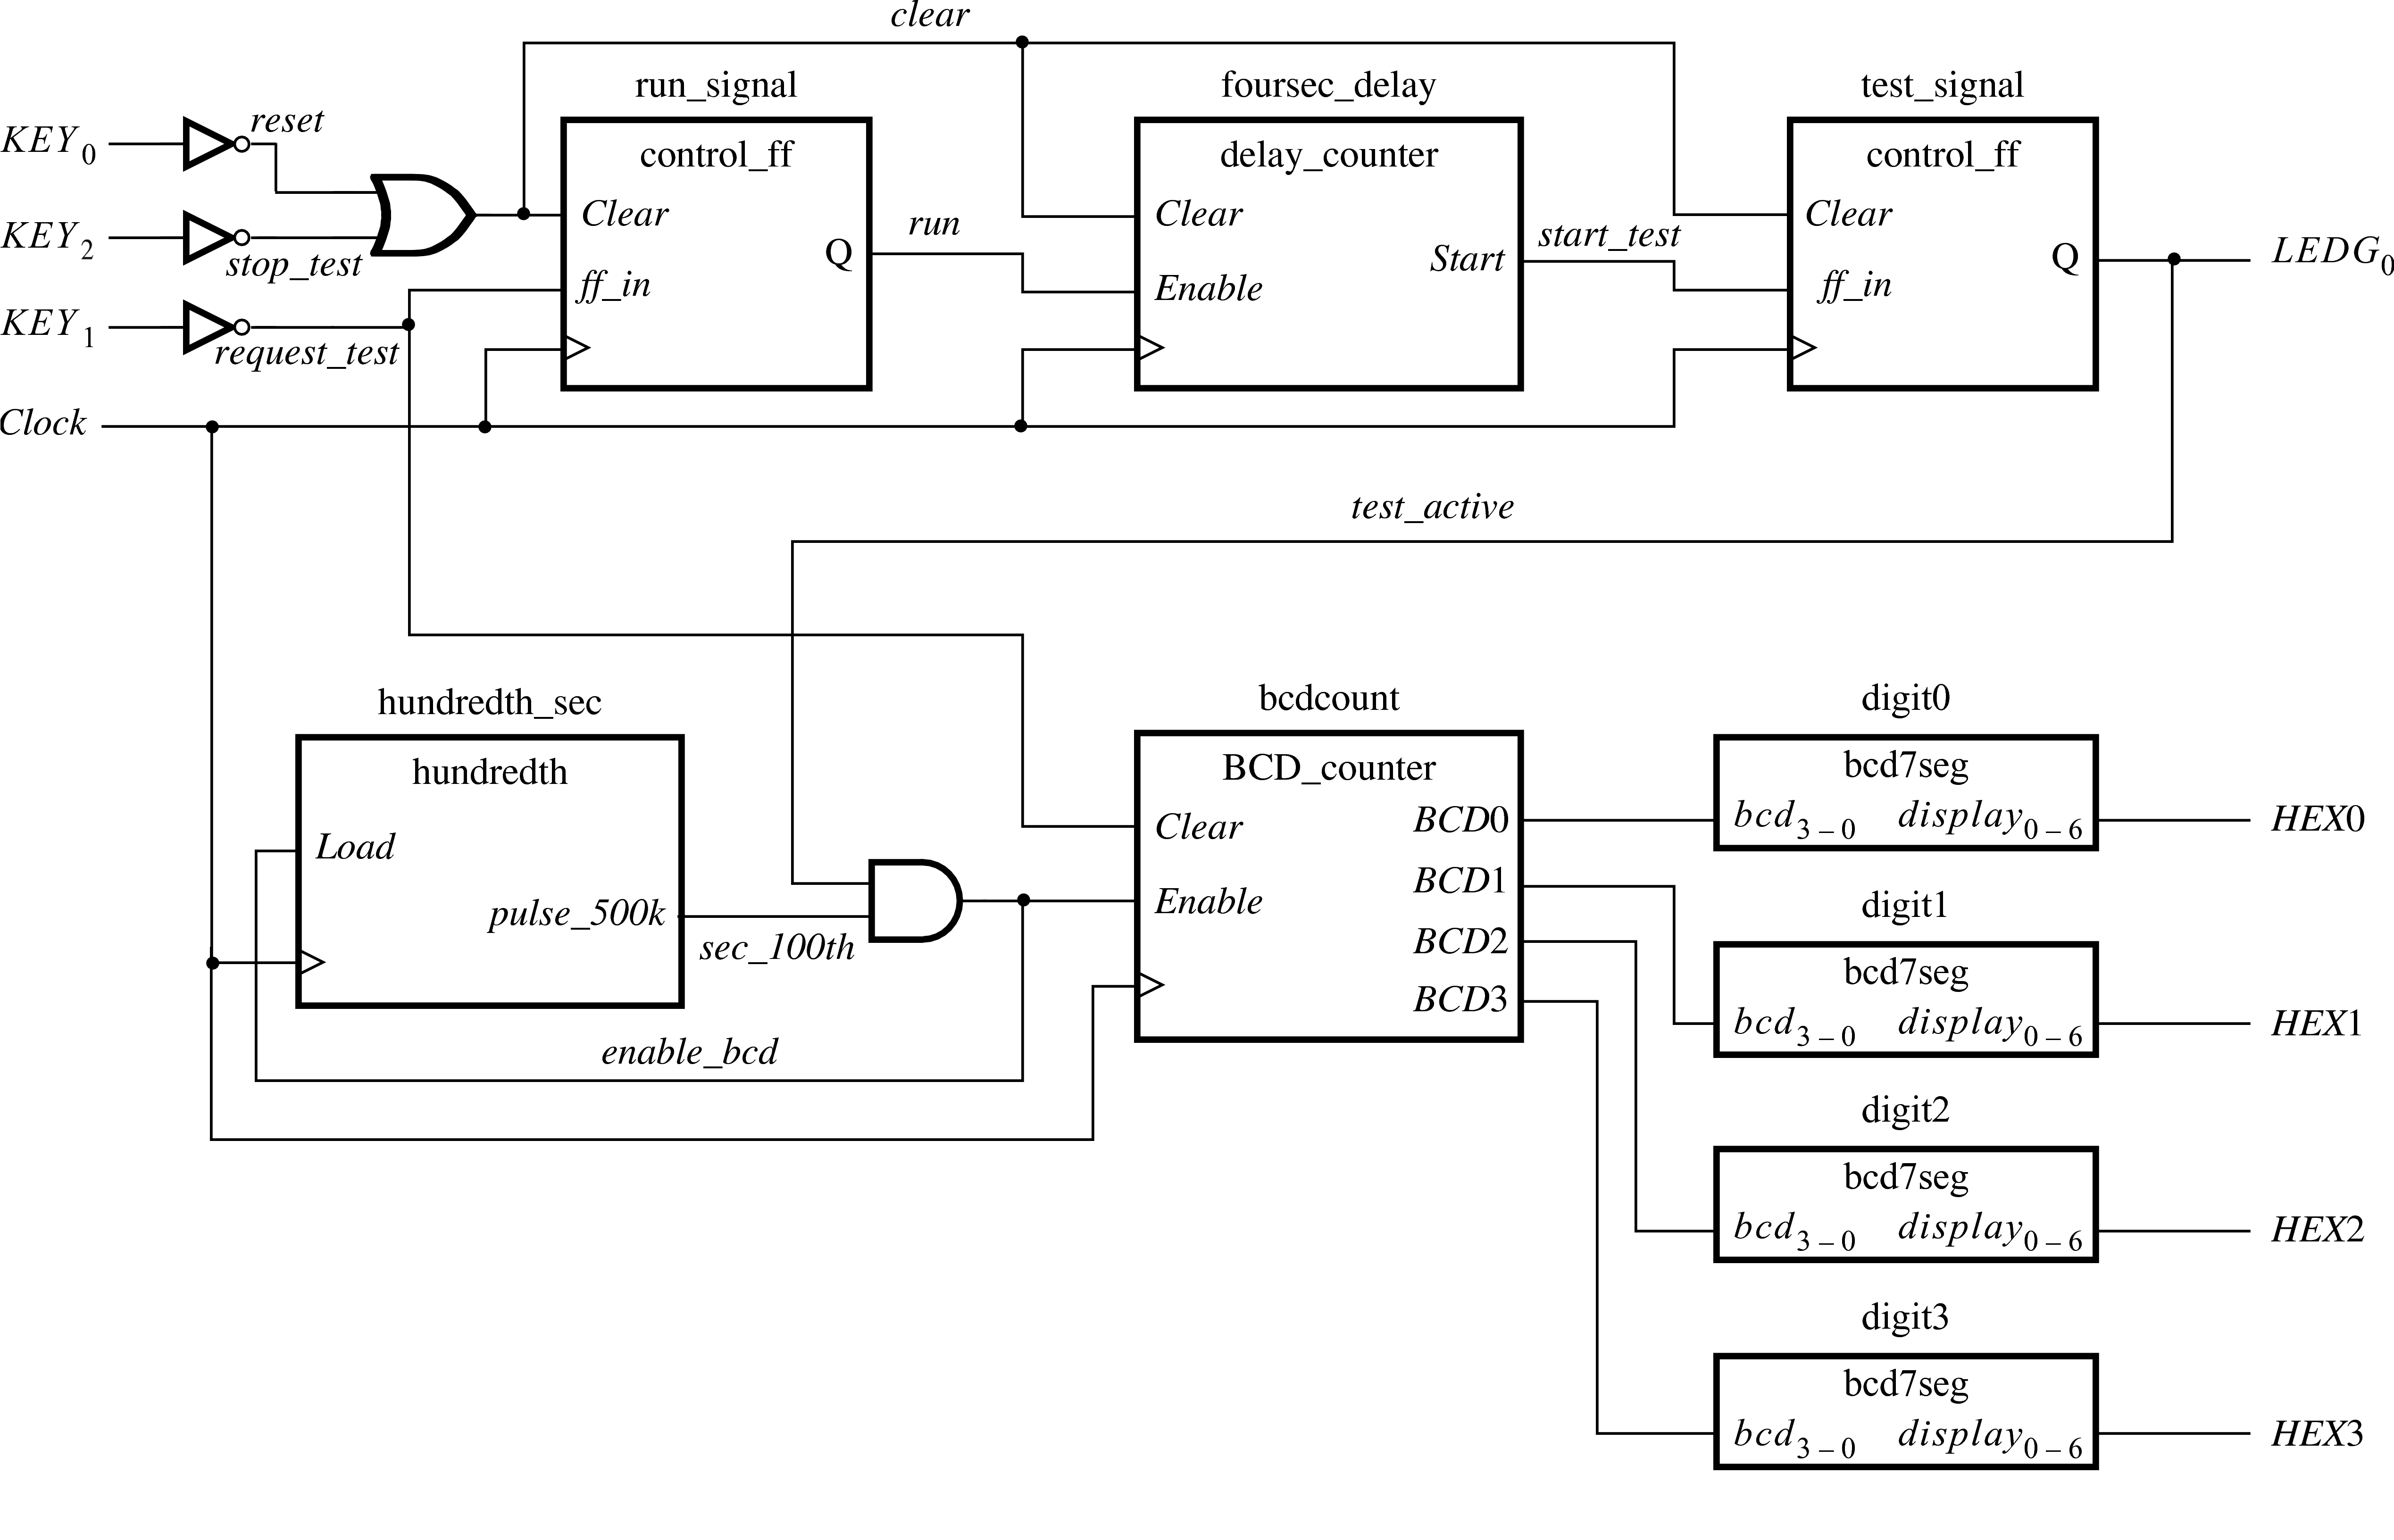
\includegraphics[scale=0.85]{figures/figure1.png}
   \caption{The reaction-tester circuit.} 
	 \label{fig:1}
	 \end{center}
\end{figure}

\begin{figure}[H]
\lstinputlisting[language=VHDL, xleftmargin=2cm, numbers=left, stepnumber=1, lastline=9]{design_files/reaction_tester/reaction_tester.vhd}
	\caption{VHDL code for the top-level module of the example system. (Part {\it a})}
	\label{fig:2}
\end{figure}

\newpage
\begin{center}
\lstinputlisting[language=VHDL, xleftmargin=0.5cm, numbers=left, stepnumber=1, firstnumber=10, firstline=10]{design_files/reaction_tester/reaction_tester.vhd}

Figure 2.  VHDL code for the top-level module of the example system. (Part {\it b})
\end{center}
~\\
The subcircuit in the {\it control\_ff} modules is defined in Figure~\ref{fig:3}.
It generates an output signal that goes high when the data input
{\it ff\_in} goes high, and then maintains this signal, even if {\it ff\_in}
becomes low again, until it is cleared by a
signal on the {\it Clear} input. Note that while the inputs may be asynchronous 
(being connected to pushbutton switches), the operation is synchronized by the 
clock signal. A circuit generated from this code is displayed in Figure~\ref{fig:4}.

\begin{figure}[H]
\lstinputlisting[language=VHDL, xleftmargin=3cm]{design_files/reaction_tester/control_ff.vhd}
	\caption{Code for the \it{control\_ff} circuit.}
	\label{fig:3}
\end{figure}

\begin{figure}[H]
   \begin{center}
      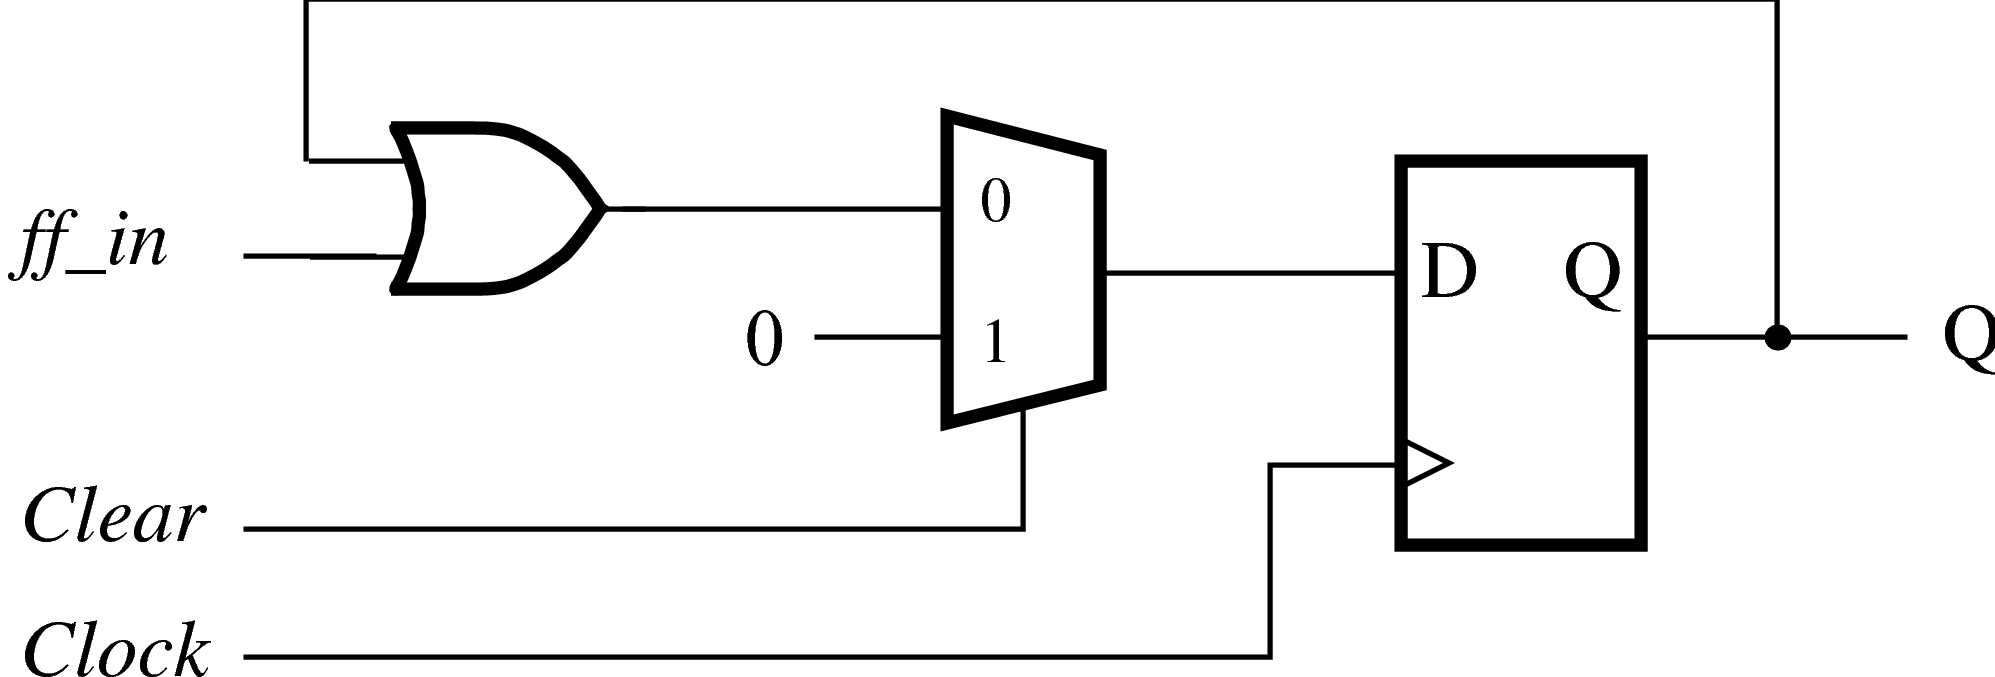
\includegraphics[scale=1]{figures/figure4.png}
   \caption{The {\it control\_ff} circuit.} 
	 \label{fig:4}
	 \end{center}
\end{figure}

Figure~\ref{fig:5} presents the code for the delay counter module, {\it delay\_counter}.
This is a 28-bit up-counter. Its most-significant bit, $b_{27}$,
goes to 1 after about four seconds. It is used as the {\it start\_test} signal.
The code produces the circuit in Figure~\ref{fig:6}. Note that the
counter is implemented as a 28-bit register (represented by the flip-flop symbol),
and an adder which increments the contents of the register by 1.

\begin{figure}[H]
\lstinputlisting[language=VHDL, xleftmargin=3cm]{design_files/reaction_tester/delay_counter.vhd}
	\caption{Code for the {\it delay\_counter} circuit.}
	\label{fig:5}
\end{figure}
 
\begin{figure}[H]
   \begin{center}
      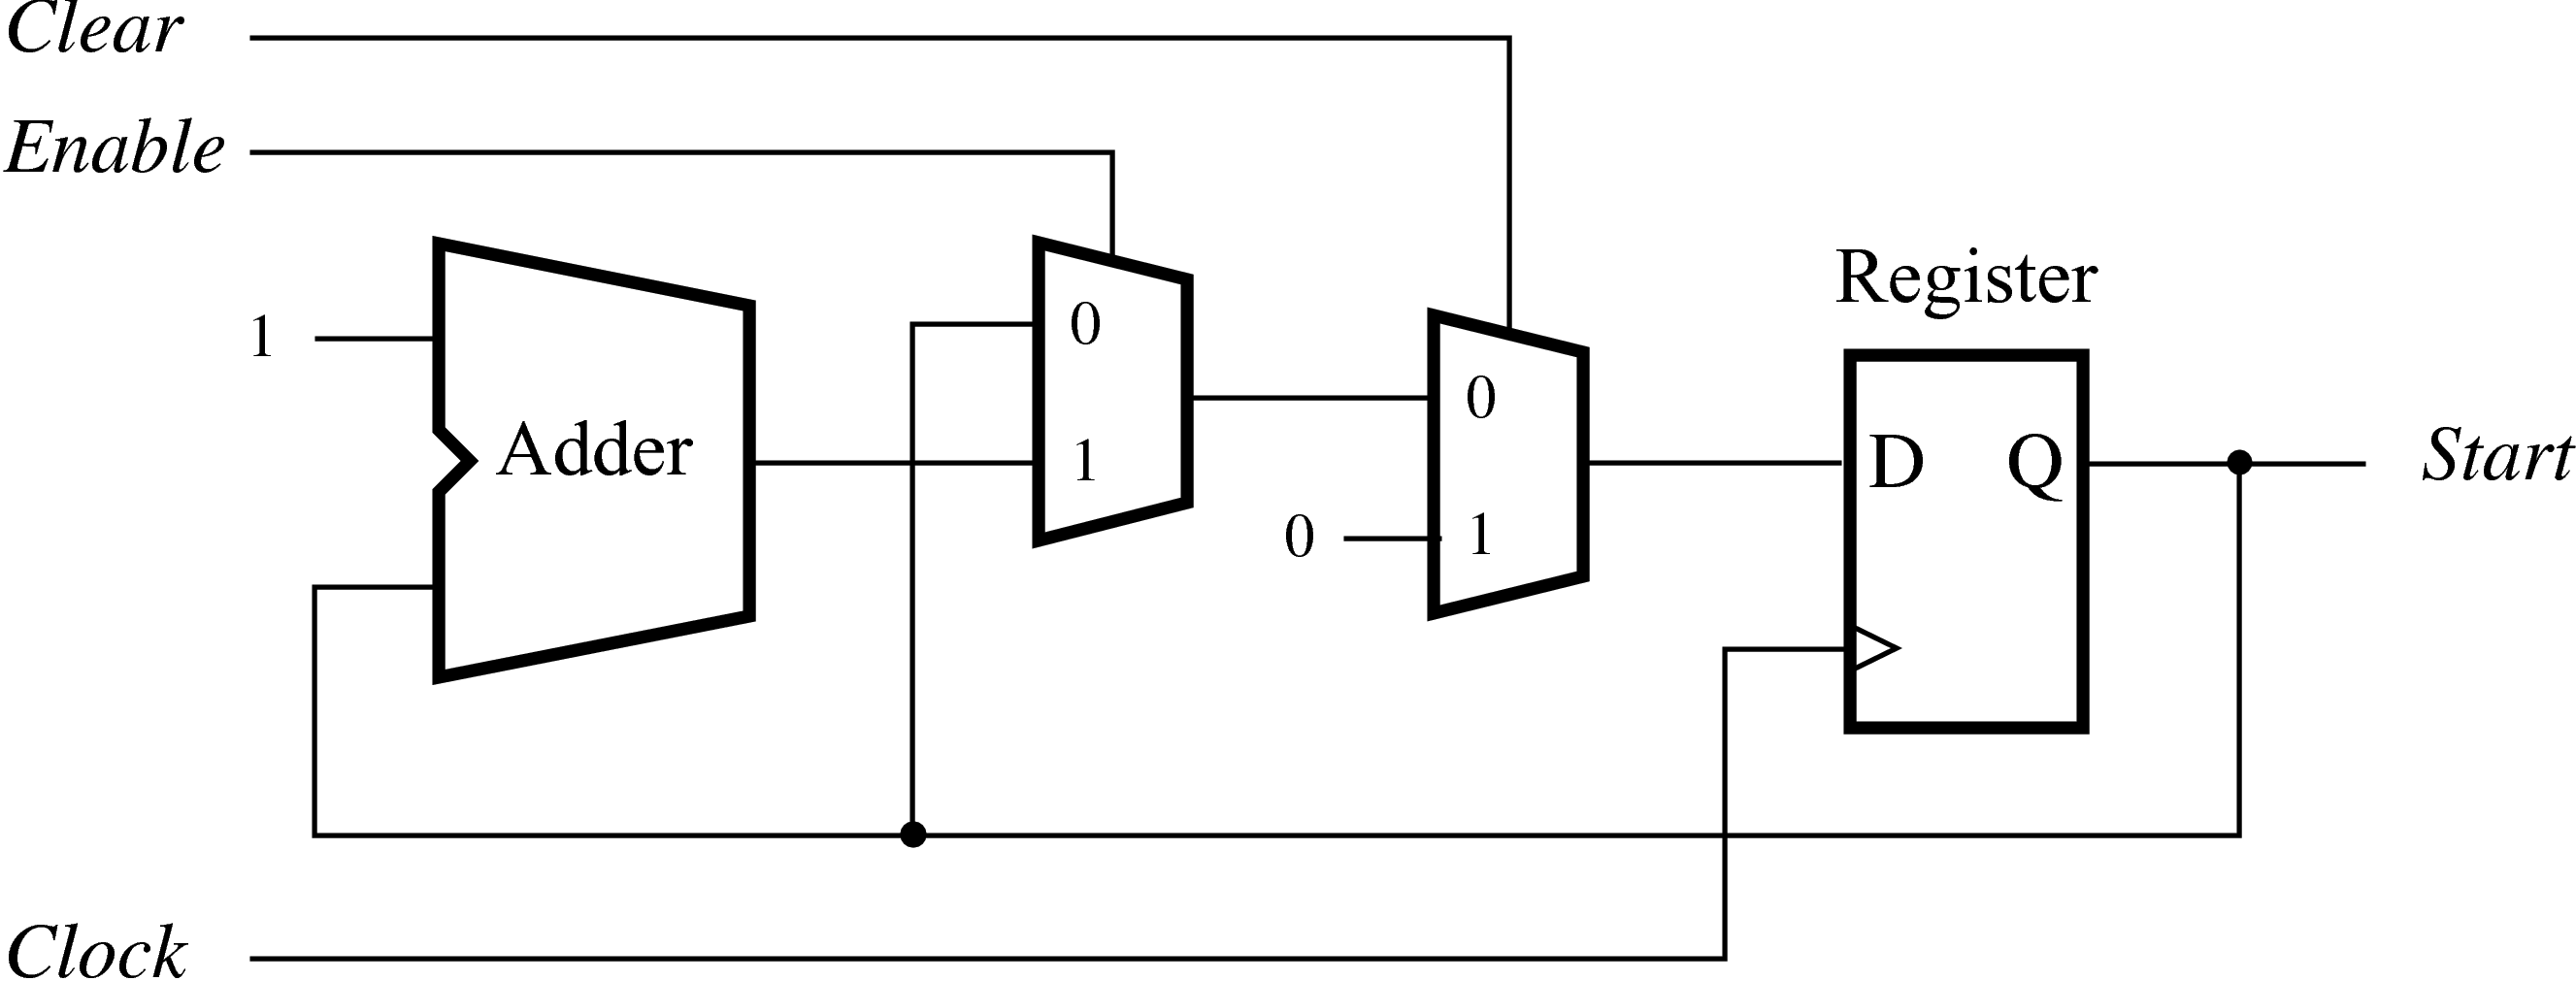
\includegraphics[scale=0.9]{figures/figure6.png}
   \caption{The {\it delay\_counter} circuit.} 
	 \label{fig:6}
	 \end{center}
\end{figure}

Figure~\ref{fig:7} gives the code that defines the {\it hundredth} subcircuit. This is a 
down-counter which generates an output pulse
whenever the contents reach the value 0. To produce the interval of one hundredth
of a second, the counter is repeatedly loaded with the value (7A120)$_{16}$ which
corresponds to 500,000. The output of this circuit, {\it sec\_100th}, allows
the BCD counter to be incremented 100 times each second
as long as the green light is on. The circuit is shown in Figure~\ref{fig:8}. This
counter is implemented as a 20-bit register (represented by the flip-flop symbol),
and an adder which decrements the contents of the register by 1.

\begin{figure}[H]
\lstinputlisting[language=VHDL, xleftmargin=3cm]{design_files/reaction_tester/hundredth.vhd}
	\caption{Code for the {\it hundredth} circuit.}
	\label{fig:7}
\end{figure}
 
\begin{figure}[H]
   \begin{center}
      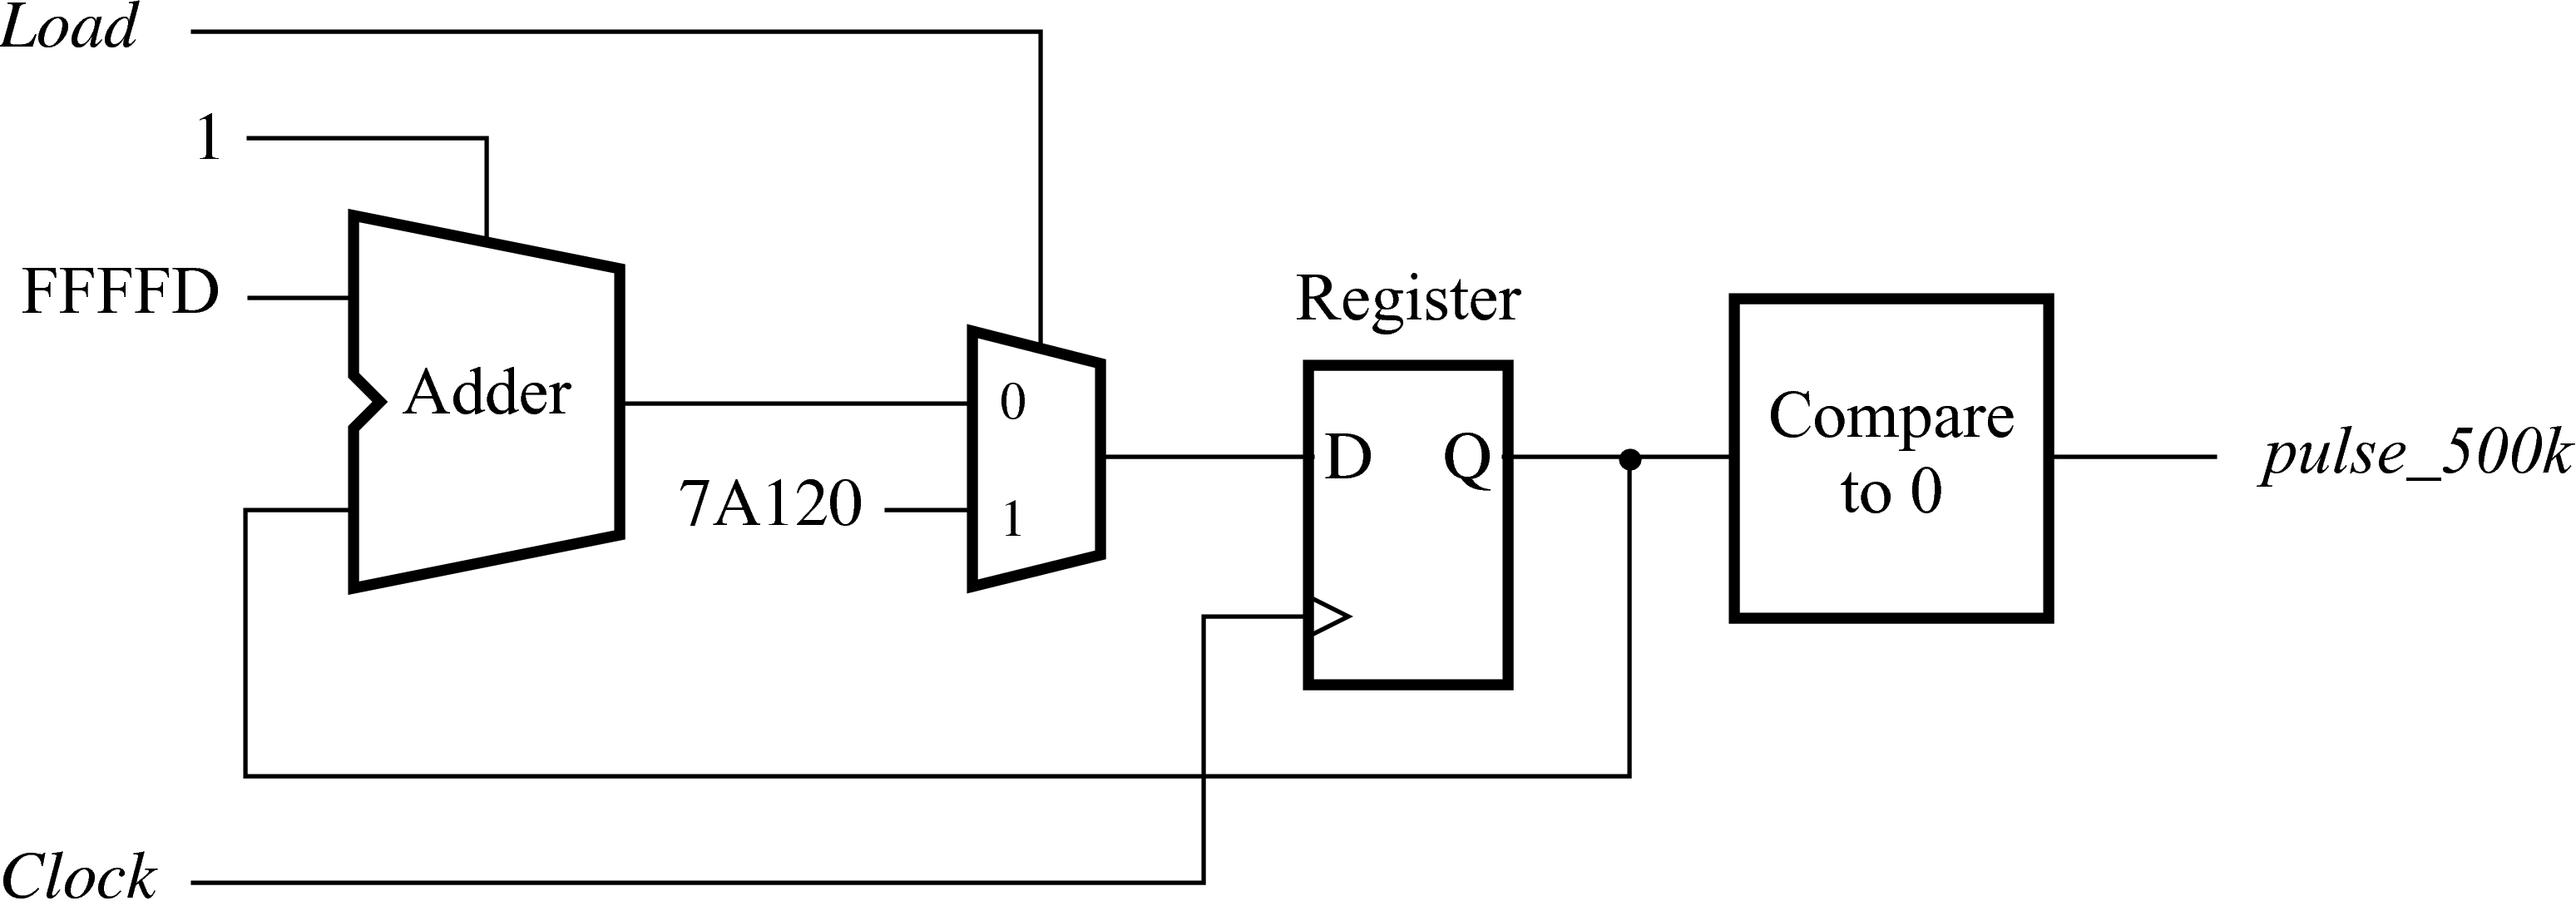
\includegraphics[scale=1]{figures/figure8.png}
   \caption{The {\it hundredth} circuit.} 
	 \label{fig:8}
	 \end{center}
\end{figure}

The BCD counter is specified by the code in Figure~\ref{fig:9}.
The circuit for each of the four BCD digits is defined in the module {\it BCD\_stage}.
Four versions of this circuit are instantiated in the module {\it BCD\_counter}.
Figures~\ref{fig:10} and~\ref{fig:11} depict the circuits synthesized from the modules {\it BCD\_counter}
and {\it BCD\_stage}, respectively.

\begin{figure}[H]
\lstinputlisting[language=VHDL, xleftmargin=0.5cm]{design_files/reaction_tester/BCD_counter.vhd}
  \vspace{-0.5cm}
	\caption{Code for the {\it BCD\_counter} circuit.}
	\label{fig:9}
\end{figure}


\begin{figure}[H]
   \begin{center}
      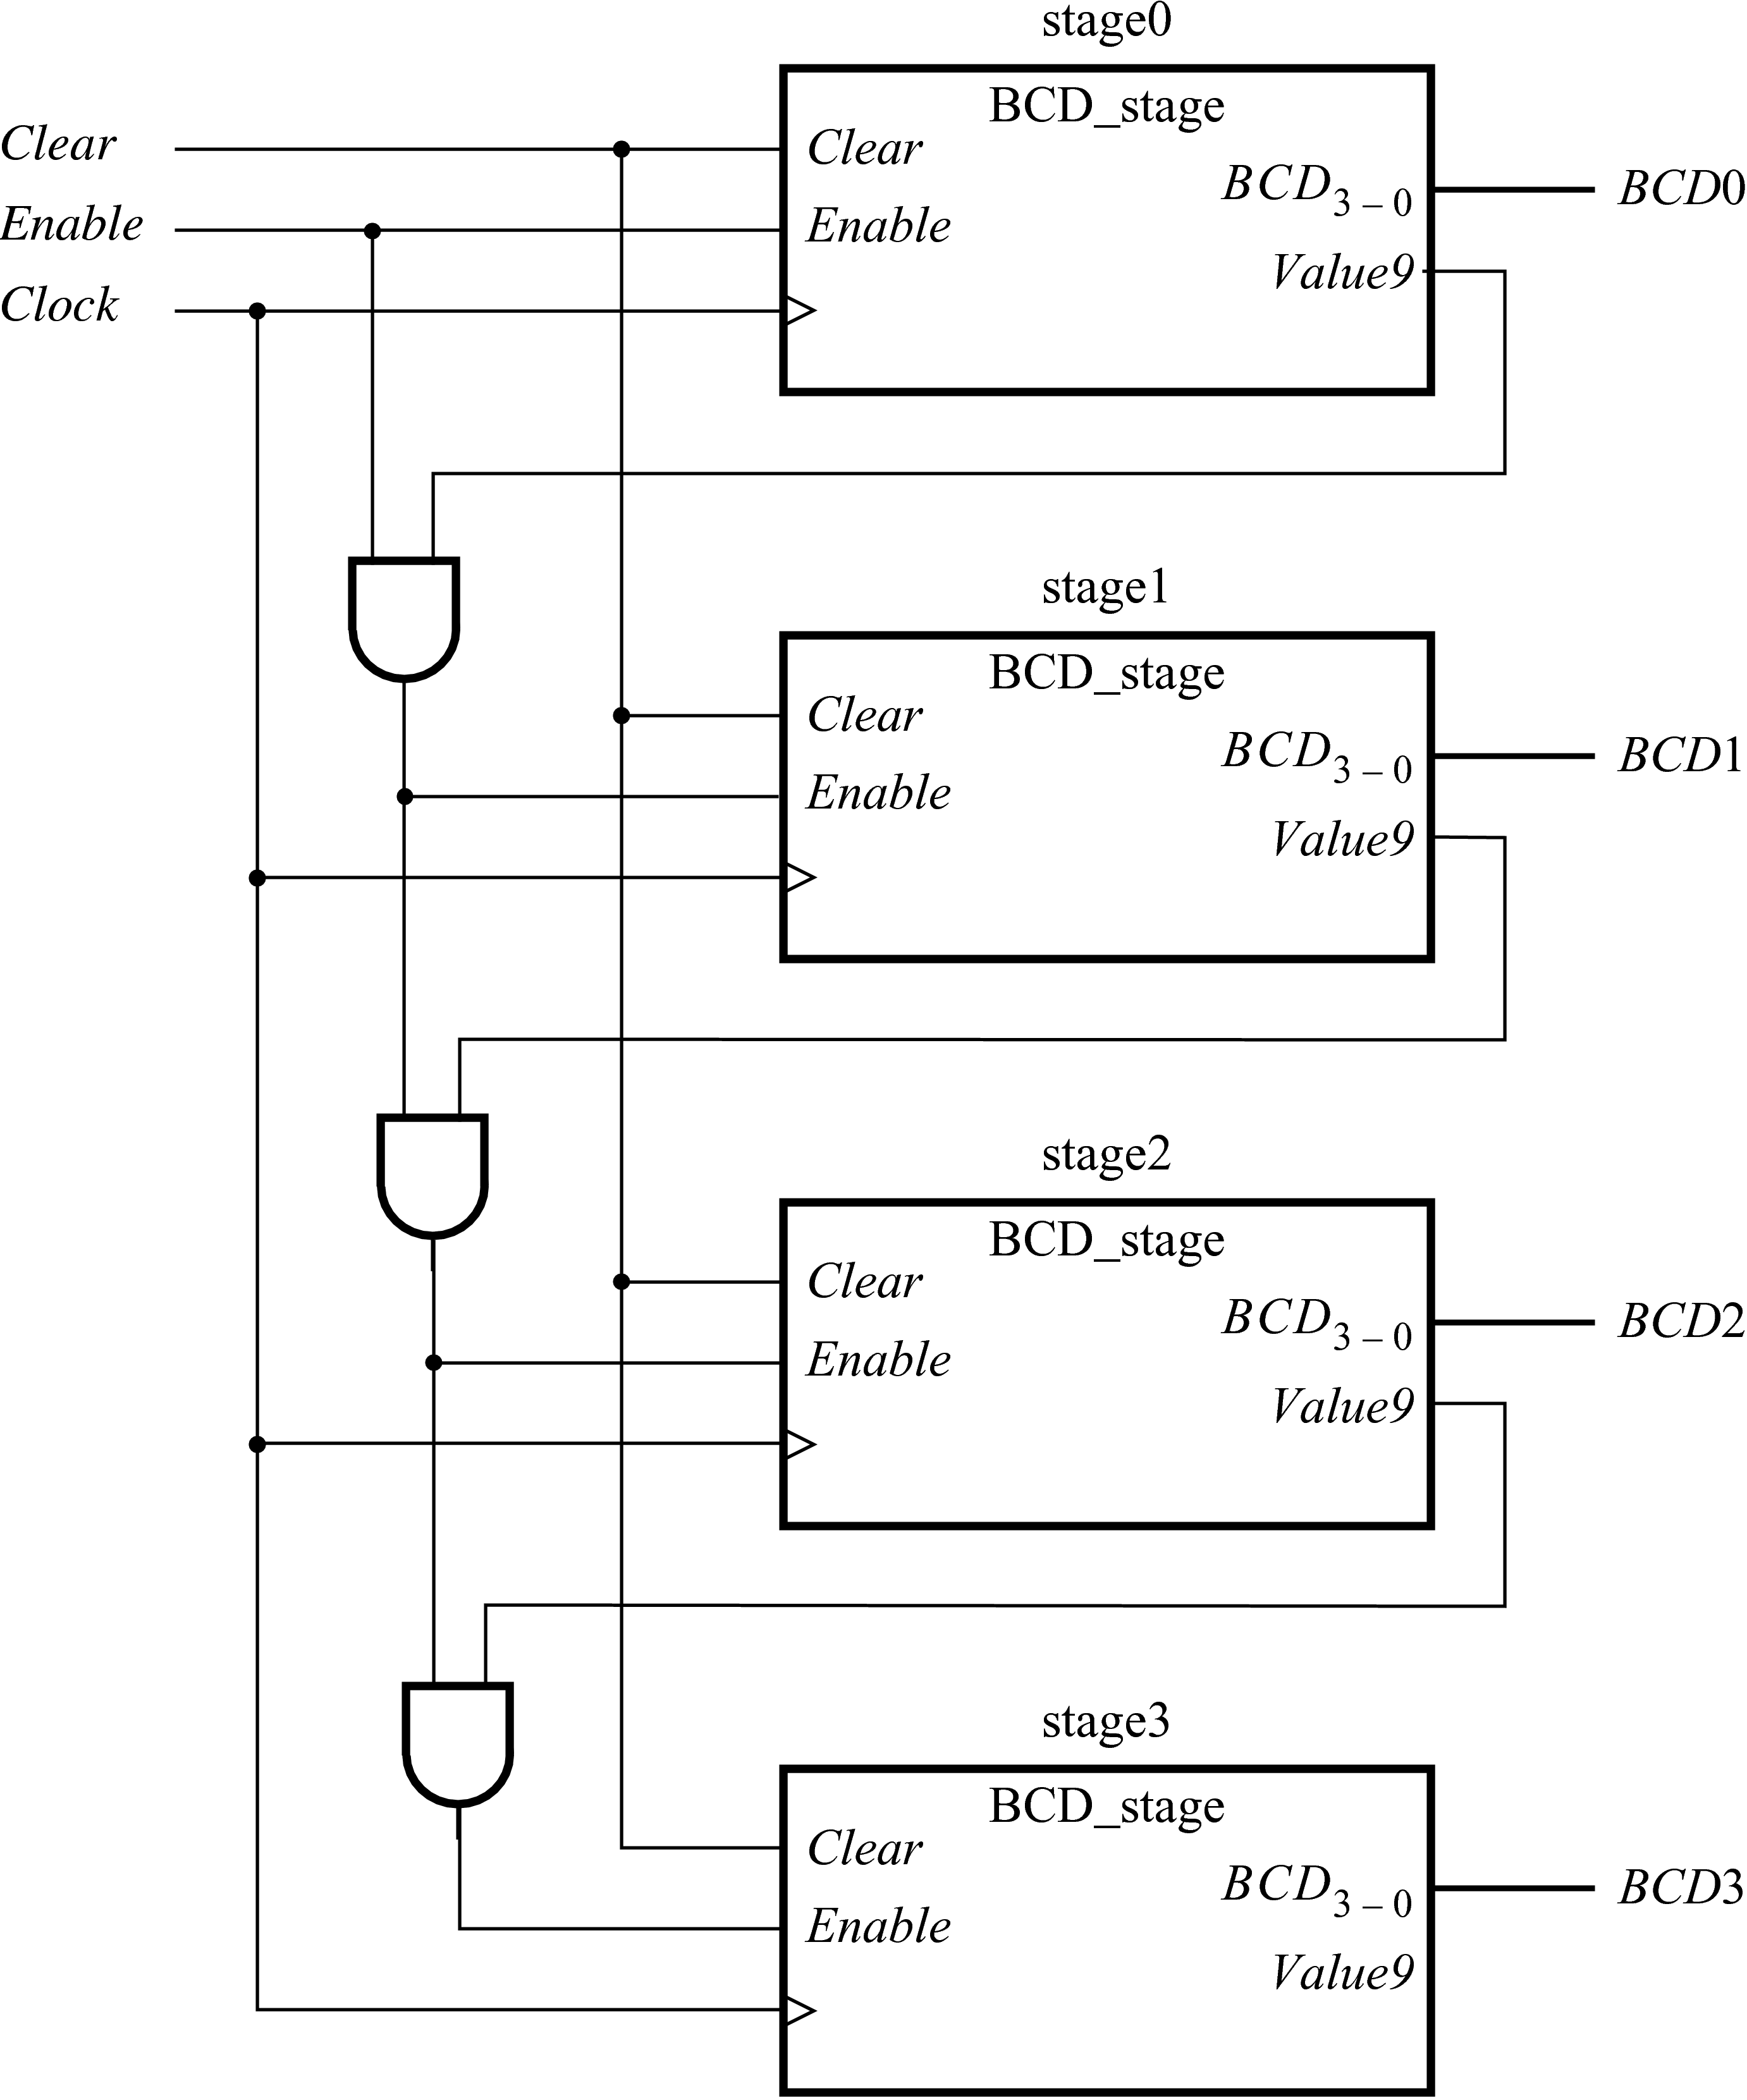
\includegraphics[scale=0.80]{figures/figure10.png}
   \caption{The {\it BCD\_counter} circuit.} 
	 \label{fig:10}
	 \end{center}
\end{figure}

\begin{figure}[H]
   \begin{center}
      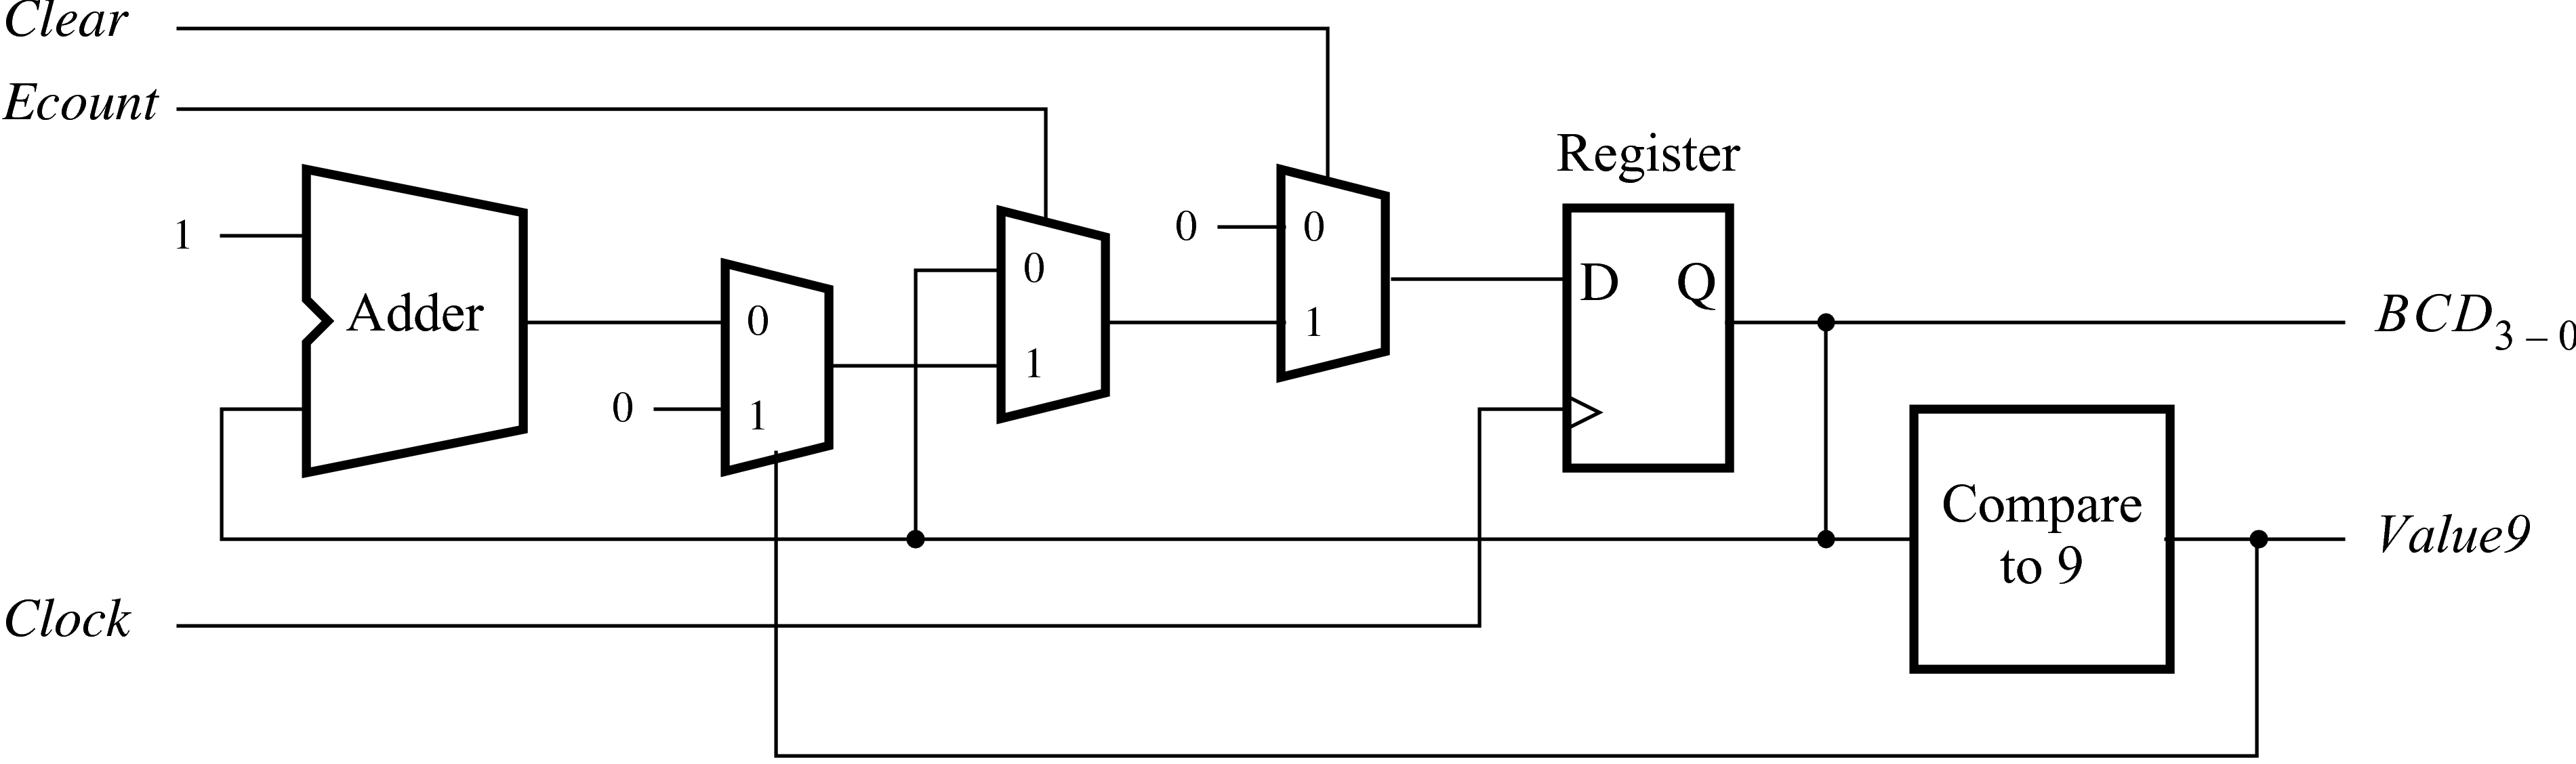
\includegraphics[scale=1]{figures/figure11.png}
   \caption{The {\it BCD\_stage} circuit.} 
	 \label{fig:11}
	 \end{center}
\end{figure}

Each digit of the BCD counter is converted into a seven-bit pattern suitable for display
on a 7-segment display on the DE-series board. This is accomplished by using the circuit 
{\it bcd7seg}, which is specified by the code in Figure~\ref{fig:12}. Note that the comment in the code 
shows the labeling of the segments that corresponds to the implementation on the DE-series board.
 
\begin{figure}[H]
\lstinputlisting[language=VHDL, xleftmargin=3cm]{design_files/reaction_tester/bcd7seg.vhd}
	\caption{Code for the BCD-to-7-segment decoder circuit.}
	\label{fig:12}
\end{figure}
 

Figure~\ref{fig:13} gives a circuit that may result from the code in Figure~\ref{fig:12}.
Each segment of the 7-segment display is driven by a signal generated
by a simple decoder from the four bits of a BCD digit. The figure shows
only a part used to drive two of the segments, {\it display}$_0$ 
and {\it display}$_6$.
Each decoder realizes the assignment indicated in Figure~\ref{fig:12}.
Note that the segments of a 7-segment display are illuminated when a ground
signal, logic 0, is applied to them. They are turned off when a high-voltage
signal, logic 1, is applied.

While Figure~\ref{fig:13} shows specific decoder circuits, it is important to keep in mind
that the Quartus Prime compiler may synthesize different looking circuits but with
the same functionality.
 
We will use our example circuit to illustrate the debugging process.
To get the most out of this tutorial, create a new Quartus Prime project,
compile the circuit, and follow the discussion by performing the various
tasks on your design. All of the files involved in the design are provided
with this tutorial. Ensure that the included Quartus Prime project is configured for the FPGA on your DE-series board, and that you have the right pin-assignment file. Pin-assignment files can be found on the University Program \href{https://www.altera.com/support/training/university/boards.html}{website}; simply navigate to the materials section of your DE-series board's page.

Before starting the discussion of debugging, we will consider some Quartus Prime 
tools that make the debugging task easier.    

\begin{figure}[H]
   \begin{center}
      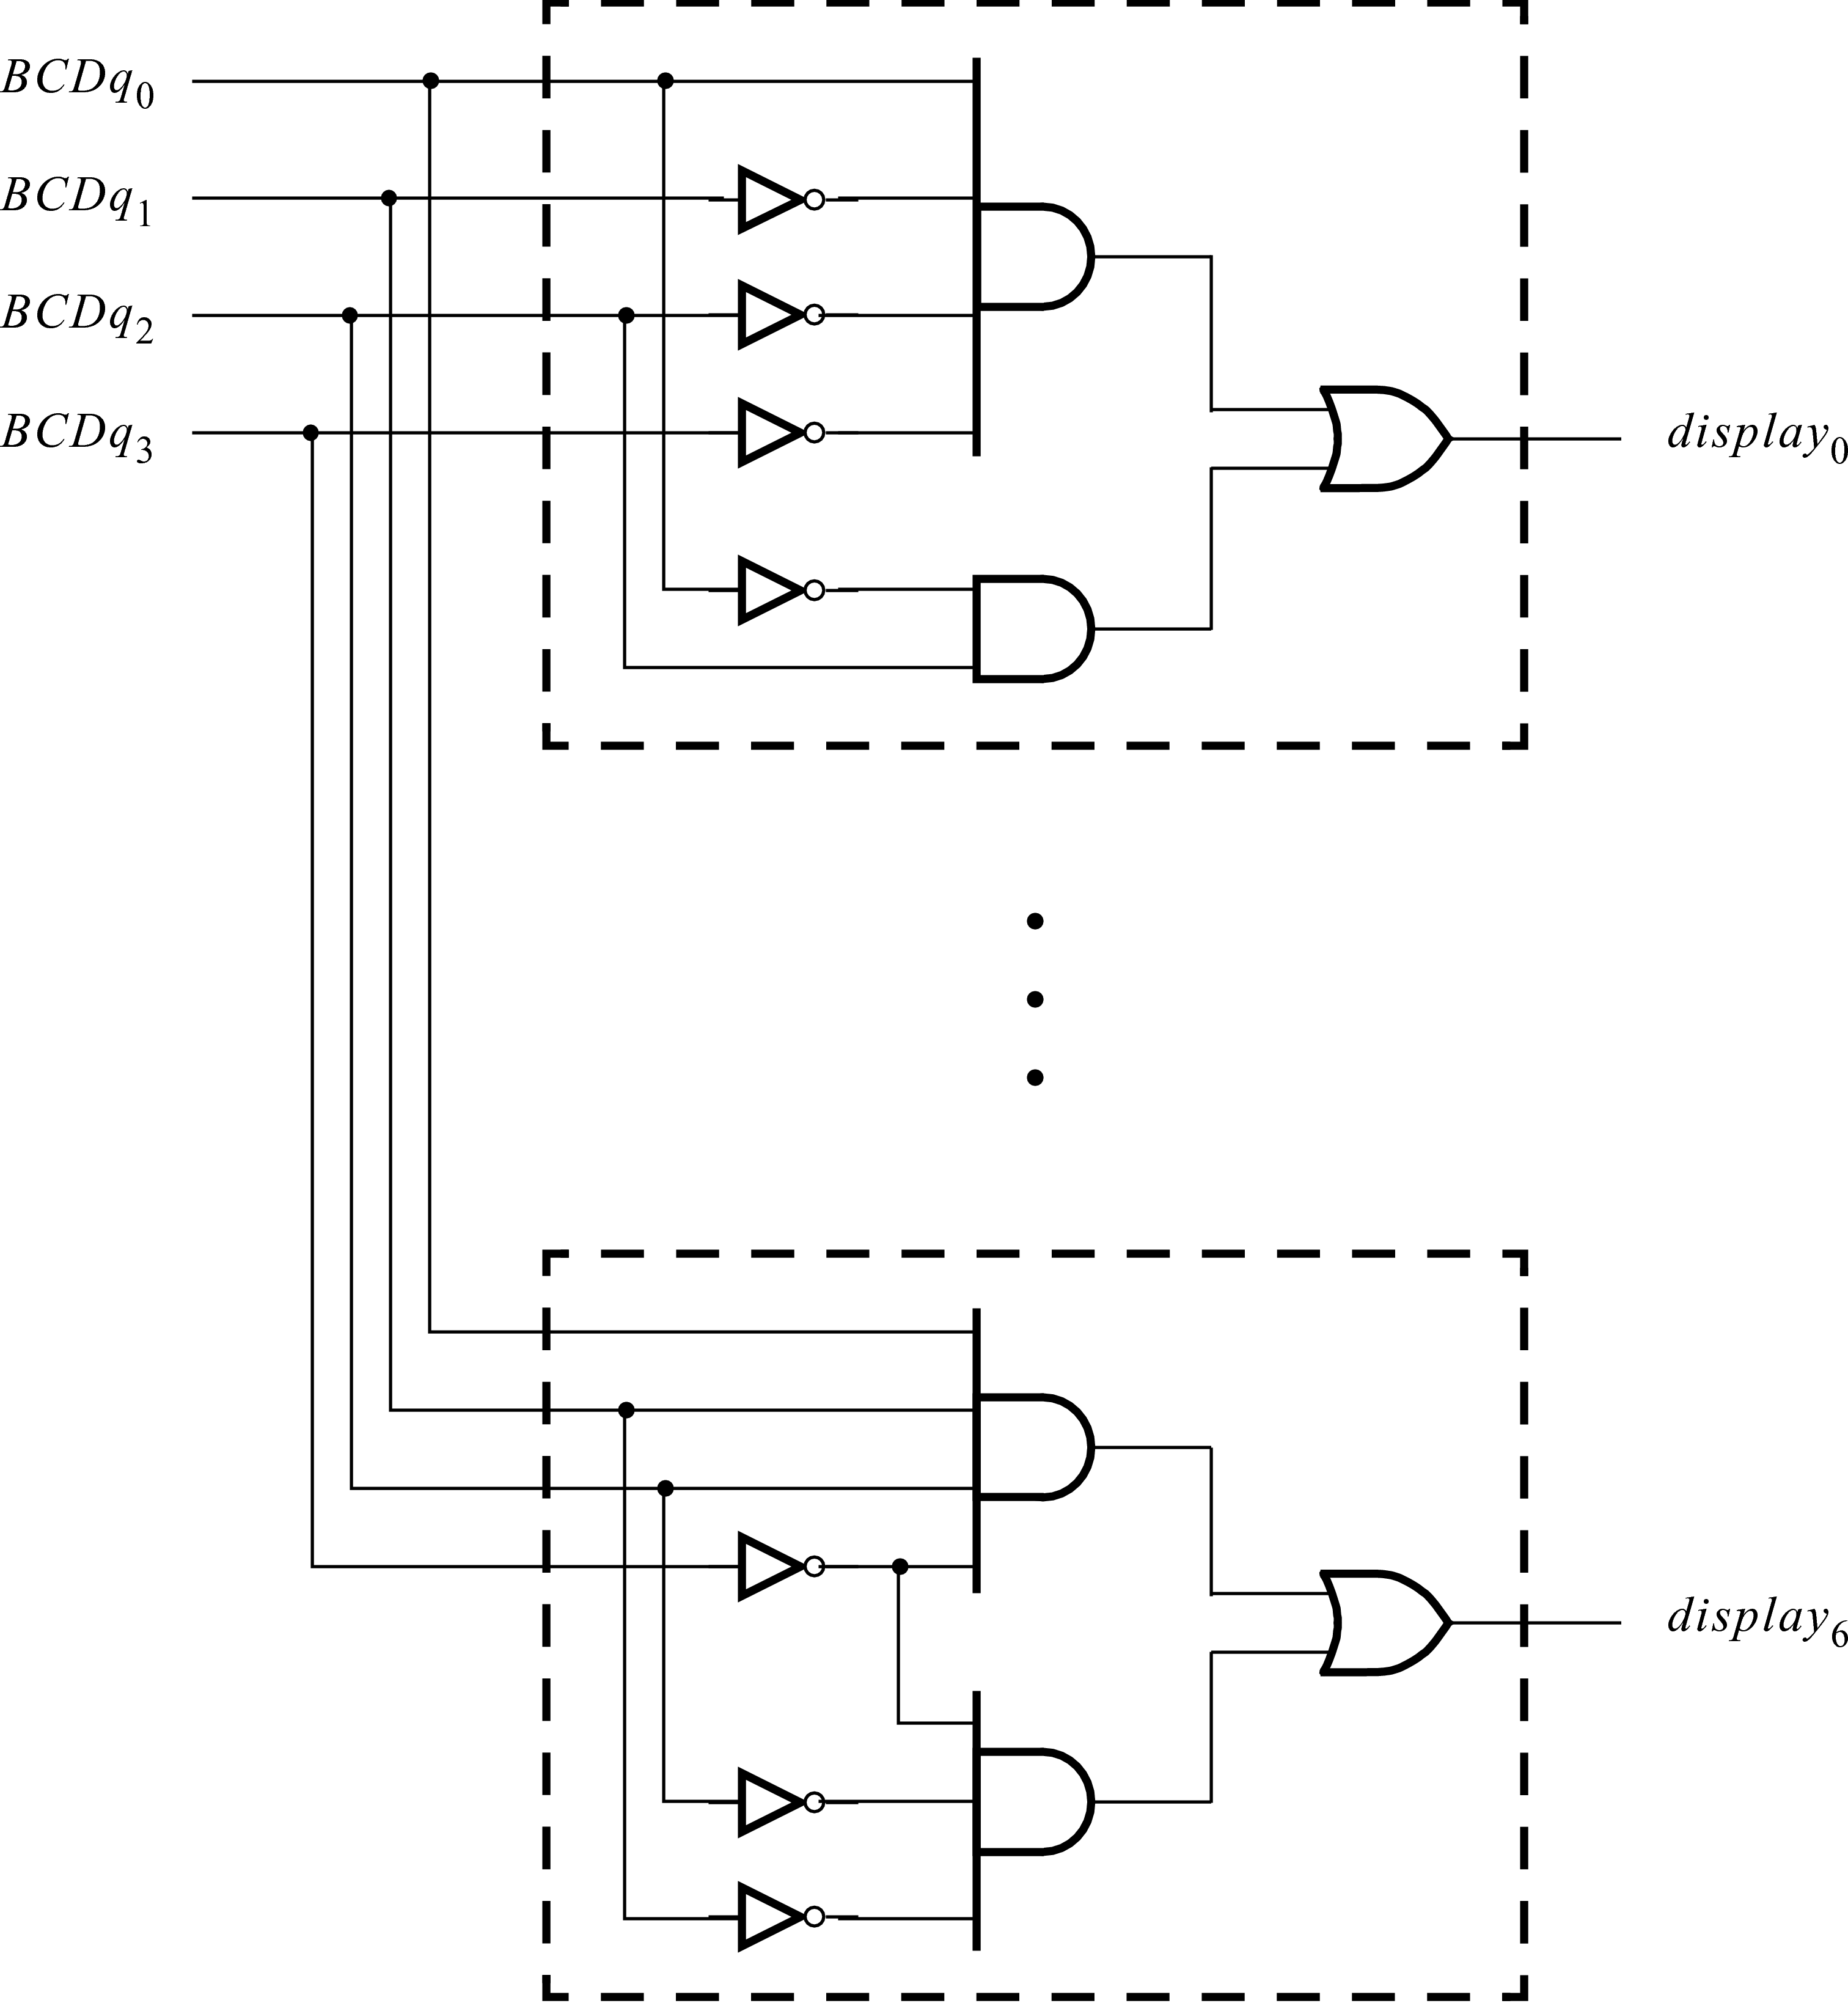
\includegraphics[scale=1]{figures/figure13.png}
   \caption{The {\it bcd7seg} circuit.} 
	 \label{fig:13}
	 \end{center}
\end{figure}

\section{Quartus\textsuperscript{\textregistered} Prime Tools for Use in Debugging of Hardware Designs}
The Quartus Prime software includes many tools that are useful for a variety
of purposes. We will discuss three types of tools: {\it Netlist Viewers},
{\it SignalTap Logic Analyzer}, and {\it Simulator}. 
While their use is broader, we will restrict
our discussion to their utility as debugging aids.

\subsection{Netlist Viewers}
The Netlist Viewers provide a graphical indication of a synthesized circuit.
A {\it register transfer level (RTL)} view of a designed circuit, generated after the
initial synthesis, can be seen by using the {\it RTL Viewer}. A view of the final 
implementation, obtained after {\it technology mapping}, is available through the
{\it Technology Map Viewer}. If a designed circuit involves a finite state machine,
a diagram of this FSM can be examined by means of the {\it State Machine Viewer}.

\subsubsection{RTL Viewer}
The RTL Viewer provides a block diagram view of a circuit, at the level of registers,
flip-flops and functional blocks that constitute the design. The displayed image
is the circuit generated after the analysis and initial synthesis steps. 
It is not necessary to wait for the rest of the compilation process to be completed, 
which includes placing and routing the designed circuit.
Using the project with our example circuit, activate the initial synthesis
process by clicking on the {\sf Start Analysis \& Synthesis} 
icon 
\includegraphics[scale=.5]{figures/icon1.png} in the toolbar.
Should this icon not be displayed in the toolbar, it can be found by selecting 
{\sf Processing $>$ Start $>$ Start Analysis \& Synthesis}, or by right-clicking
the toolbar area and selecting {\sf Standard} to make the icon appear. Upon performing the synthesis, select
{\sf Tools $>$ Netlist Viewers $>$ RTL Viewer} to reach the window depicted in Figure~\ref{fig:14}. 
%This shows a portion of the designed circuit.
%The rest of the circuit can be examined by scrolling through this window.
The view of the circuit can be enlarged or reduced by means of the Zoom Tool. The complete
circuit is given in Figure~\ref{fig:15}.

\begin{figure}[H]
   \begin{center}
      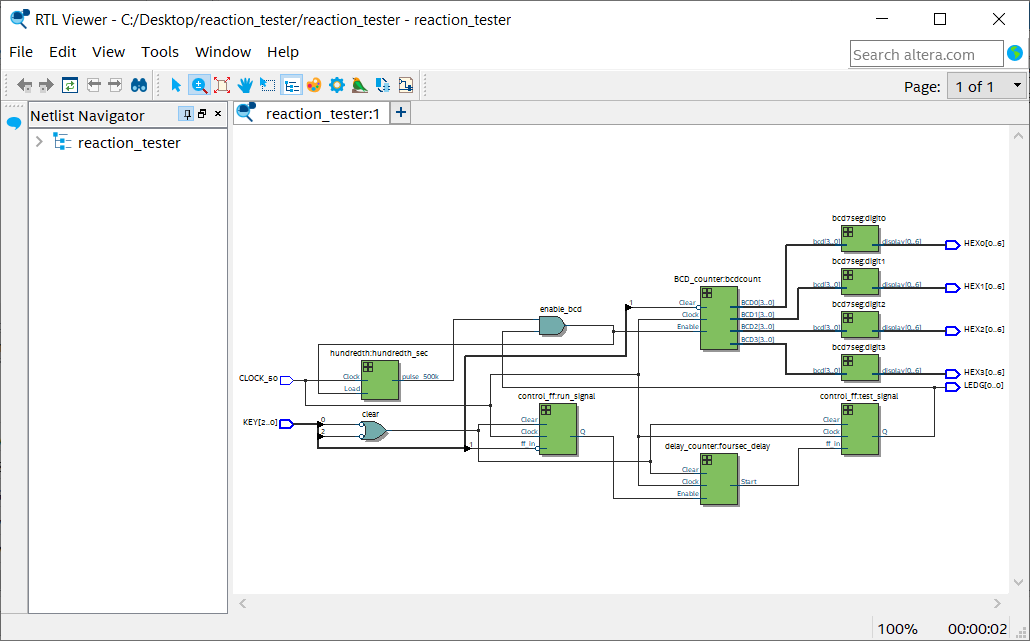
\includegraphics[scale=0.7]{figures/figure14.png}
   \caption{The RTL Viewer.} 
	 \label{fig:14}
	 \end{center}
\end{figure}

\begin{figure}[H]
   \begin{center}
      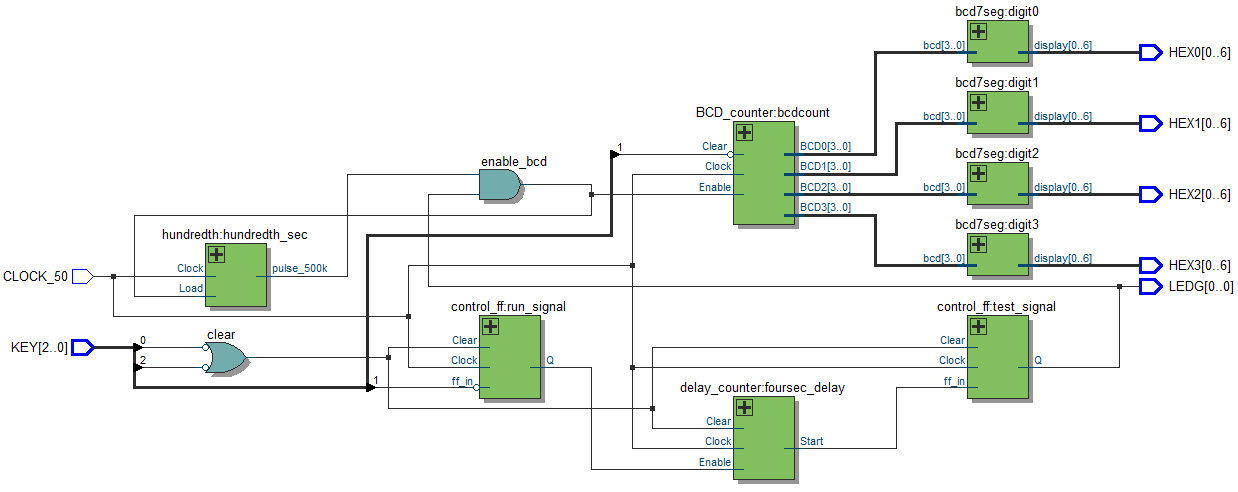
\includegraphics[scale=0.45]{figures/figure15.png}
   \caption{The complete RTL view of the {\it reaction-tester} circuit.} 
	 \label{fig:15}
	 \end{center}
\end{figure}

Double-clicking on any block of the displayed circuit will reveal a more detailed
structure of this block. For example, doing this on the block labeled
"control\_ff:run\_signal" produces the image in Figure~\ref{fig:16}. This is the circuit that
we anticipated in Figure~\ref{fig:4}.

\begin{figure}[H]
   \begin{center}
      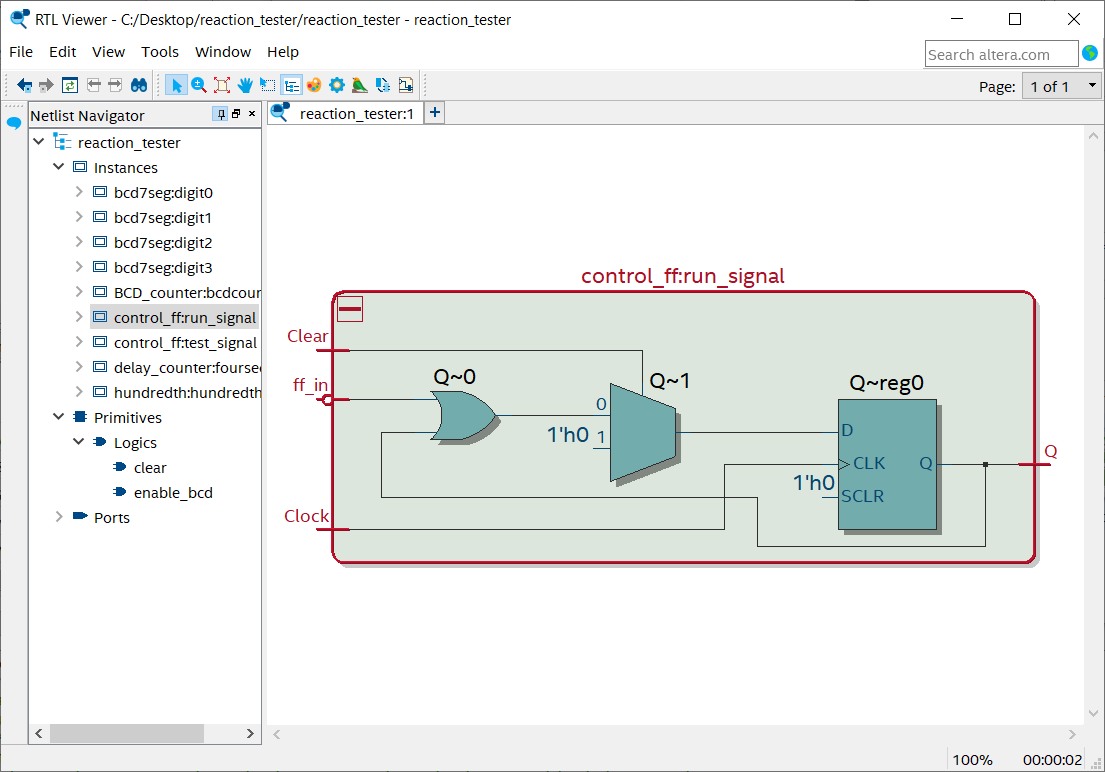
\includegraphics[scale=0.55]{figures/figure16.png}
   \caption{The RTL Viewer presentation of the {\it control\_ff} circuit.} 
	 \label{fig:16}
	 \end{center}
\end{figure}

The RTL Viewer is a very useful debugging aid. It allows the designer to quickly see
the structure of the circuit that is being designed. It shows the connections between
functional blocks. Names of the signals on the connecting wires can be seen by
hovering the mouse over the wires, which makes it easy to trace the signals. 
The displayed diagram includes only those circuit
blocks that are driven by valid inputs and produce outputs that connect to other
blocks or pins on the FPGA device. Thus, if an expected block is missing, it is 
very likely that the VHDL specification of the corresponding inputs or outputs
is incorrect.

Since the RTL Viewer displays the circuit obtained after the initial synthesis
(without needing to perform a complete compilation), it takes relatively little time 
to see the effect of any changes that are made in the design. 

\subsubsection{Technology Map Viewer}
The Technology Map Viewer can be used to examine a circuit that was compiled.
It displays not only the structure of the circuit, but it also indicates
the details of logic cells that are used to implement the various parts of the circuit.
It is activated by selecting {\sf Tools $>$ Netlist Viewers $>$ Technology Map Viewer (Post-Fitting)}.
Figure~\ref{fig:17} shows a portion of the displayed image for our example circuit.
Double-clicking on a particular block displays the details of the block.

The displayed image indicates how the designed circuit is implemented in a specific
technology. On the DE-series board this is the technology of the Cyclone\textsuperscript{\textregistered} series FPGA.

\begin{figure}[H]
   \begin{center}
      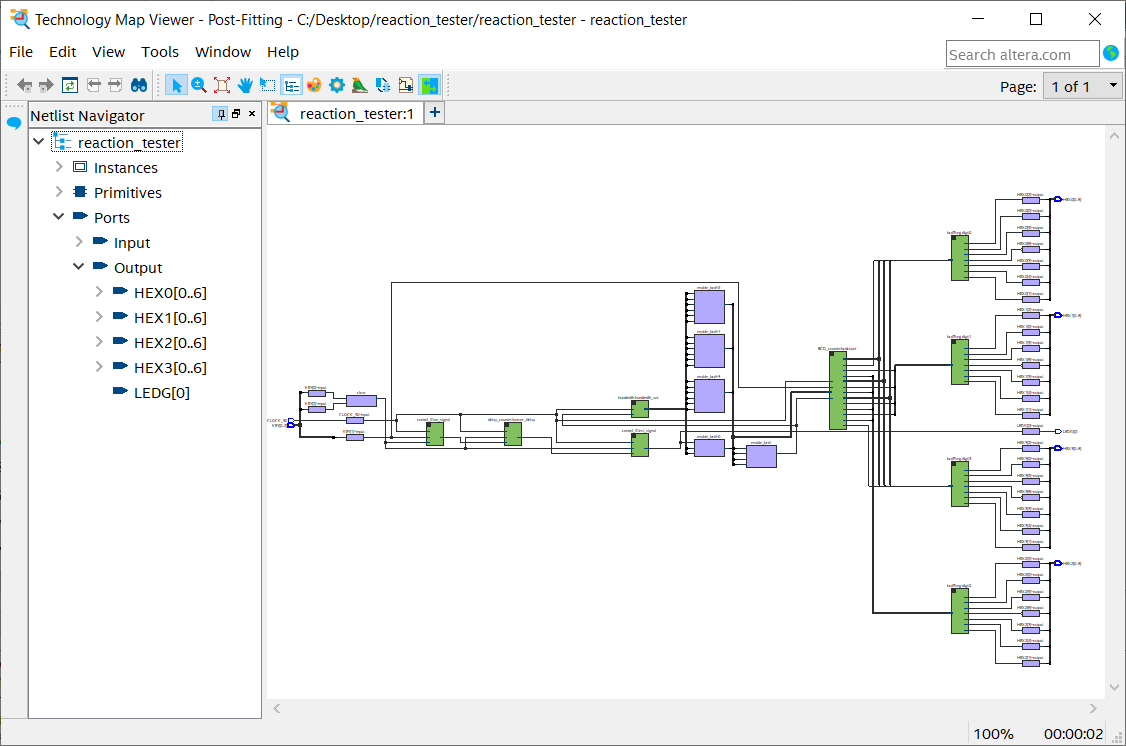
\includegraphics[scale=0.6]{figures/figure17.png}
   \caption{The Technology Map Viewer.} 
	 \label{fig:17}
	 \end{center}
\end{figure}

\subsubsection{State Machine Viewer}
If a state machine exists in your design, the State Machine Viewer can be used to examine the implementation of FSMs that are
a part of a designed circuit. It is accessed by selecting
{\sf Tools $>$ Netlist Viewers $>$ State Machine Viewer}.

The FSM implementation is depicted in both graphical and tabular forms.
The encoding of states is also presented. 

\subsection{SignalTap Logic Analyzer}
A traditional Logic Analyzer is an instrument that can display waveforms that
correspond to signals obtained by connecting probes to various points in an
implemented circuit. For an FPGA device, it is only possible to gain such access
to external pins. However, Quartus Prime software includes a software-implemented tool 
that acts as a virtual logic analyzer, which allows the user to examine signals
that are going to occur anywhere within a circuit implemented in an FPGA chip. 
It is called the SignalTap II Embedded Logic Analyzer. Its use is described in the
tutorial {\it SignalTap II with VHDL Designs}.

Figures~\ref{fig:18} and~\ref{fig:19} indicate how the analyzer may be used on our example
circuit. We chose to look at several signals that are affected by the
{\it start\_test} signal going to 1. As seen in Figure~\ref{fig:18}, a positive edge
of this signal is enabled as the trigger that causes the analyzer to take a 
snapshot of signal activity. Figure~\ref{fig:19} shows the waveforms that occur at
trigger time. Observe that the {\it test\_active} signal goes to 1 in the
next clock cycle (as expected). Also, observe that the contents of the
{\it hundredth} counter, called {\it count\_500k} in Figure~\ref{fig:7}, are decremented
by 1 in each clock cycle.

It is important to know that the Quartus Prime Compiler will not necessarily 
preserve the exact names of signals in combinational logic as defined in a VHDL
design file. Also, when the Node Finder is used to find signals that the
designer wants to include in the Setup window of the SignalTap Logic Analyzer,
many signals that are not registered or found on the FPGA pins may not be listed.
It is possible to force the listing of a particular signal under its original name
by means of the "keep" option, which is invoked by defining the attribute {\it keep}. 
For example, we can ensure that the {\it run} and 
{\it enable\_bcd} signals will be preserved and listed by inserting in the code in 
Figure~\ref{fig:2} the following statements:
\begin{center}
\begin{tabular}{c}
\begin{lstlisting}[language=VHDL]
ATTRIBUTE keep: BOOLEAN ;
ATTRIBUTE keep OF run: SIGNAL IS true ;
ATTRIBUTE keep OF enable_bcd: SIGNAL IS true ;
\end{lstlisting}
\end{tabular} 
\end{center}

\noindent
Using the keep option may result in a slightly different circuit
being synthesized. The circuit will have the same functionality as the intended
circuit, but it may have a slightly different timing behavior. Therefore, upon
successful completion of the debugging (or simulation) task, the modifications
inserted to invoke the keep option should be removed. 

\begin{figure}[H]
   \begin{center}
      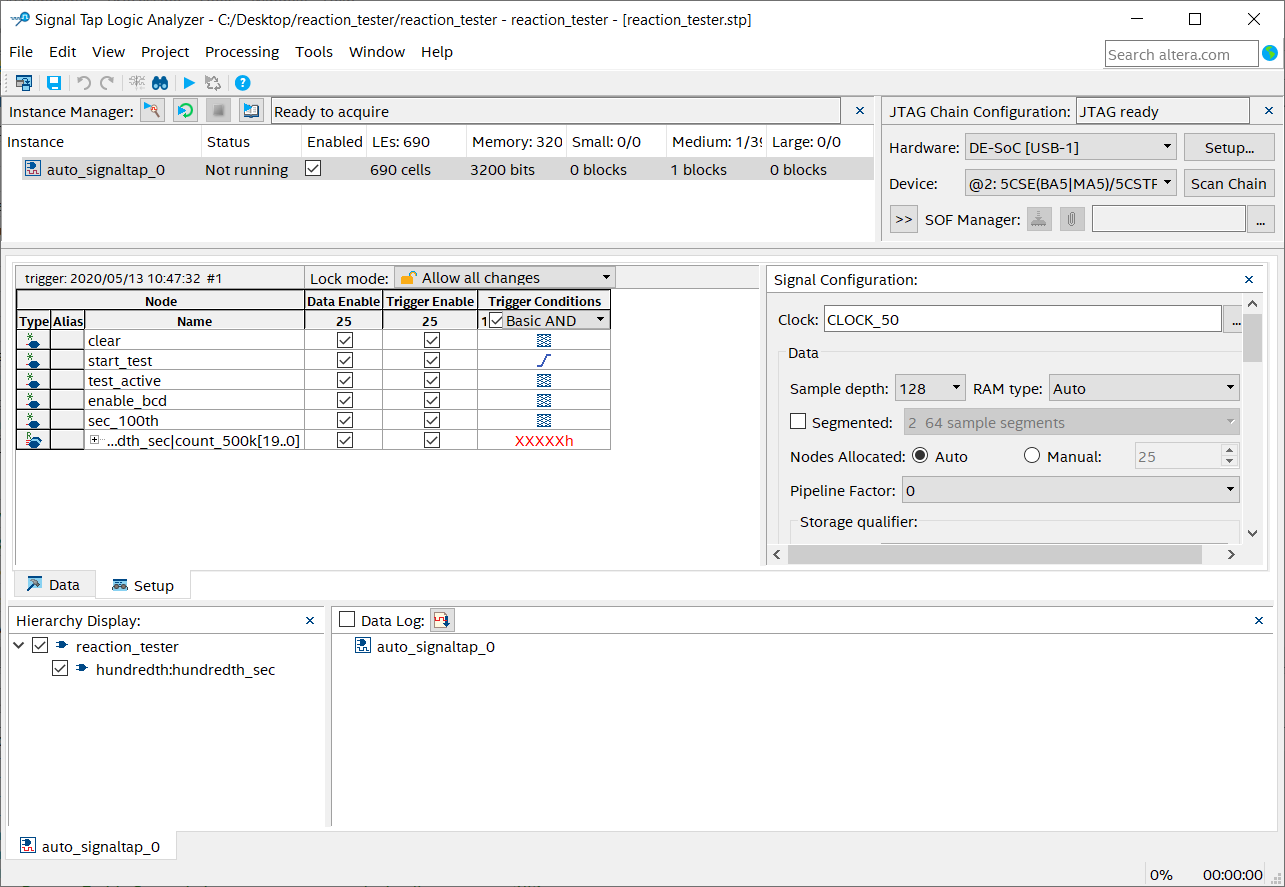
\includegraphics[scale=0.55]{figures/figure18.png}
   \caption{The Setup window of SignalTap Logic Analyzer.} 
	 \label{fig:18}
	 \end{center}
\end{figure}

\begin{figure}[H]
   \begin{center}
      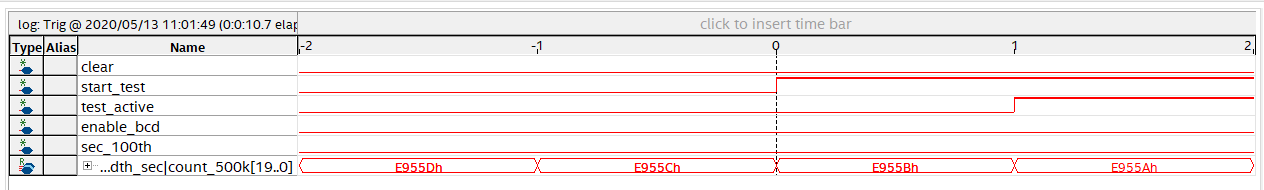
\includegraphics[scale=0.55]{figures/figure19.png}
   \caption{The Data window of SignalTap Logic Analyzer.} 
	 \label{fig:19}
	 \end{center}
\end{figure}

\subsection{Simulators}
The tools discussed above are very useful in determining whether or not a
given circuit appears to have the desired structure and functionality.
To test the expected functional correctness and performance of the designed
circuit it is useful to simulate the circuit. For example, a circuit that
performs extensive arithmetic operations may appear to be designed correctly
in terms of the components it contains, but a small error in detail (which 
could be difficult to detect using either a netlist viewer or the logic analyzer)
can cause wrong results to be produced when a particular operation is performed.
Functional simulation provides an excellent vehicle for ascertaining that the
circuit performs correctly as far as its functionality is concerned. It is
also important to ensure that the timing behavior of the circuit meets the
specification requirements, which can be determined by means of timing simulation.

A complete simulation of our example circuit would require a large number of
clock cycles, making it difficult to produce an informative display.
However, we can perform a meaningful simulation by scaling down 
some parameters. For example, let us reduce the {\it delay\_counter} circuit
to be a 4-bit counter so that the {\it start\_test} signal will go to 1 after
a delay of 8 clock cycles. Let us also reduce the {\it hundredth} counter
to be a 3-bit counter into which the value 4 is loaded whenever the {\it Load}
signal is active. A functional simulation of this scaled-down circuit is
shown in Figure~\ref{fig:20}.

We applied the input signals that correspond to the pushbutton keys. The observed
behavior of the simulated circuit is correct. The BCD counter evaluates correctly
the number of {\it sec\_100th} pulses that occur before the {\it KEY}$_2$
signal goes to 0 (which corresponds to pressing of the pushbutton).
The BCD-to-7-segment decoders also correctly decode the BCD digits, which
is easily verified by examining the displayed patterns.

Remember to invoke the "keep" option on the appropriate signals in lines 11 to 13 in Figure~\ref{fig:2}
by defining the attribute {\it keep}.

The simulation indicates that our circuit produces a slightly inaccurate result.
Before the test starts, the {\it hundredth} counter runs in a counting span
of 8 clock cycles, as shown by the {\it sec\_100th} signal in Figure~\ref{fig:20}.
During the test this span becomes 4 cycles, because this is
the value repeatedly loaded into the counter. However, at the very beginning of
the test the counter may contain the value 7, which means that it will take 8
clock cycles before the BCD counter starts counting. This means that our tester
circuit may be wrong by 1/100th of a second. If we could not tolerate this
inaccuracy, we would have to modify the circuit.

\begin{figure}[H]
   \begin{center}
      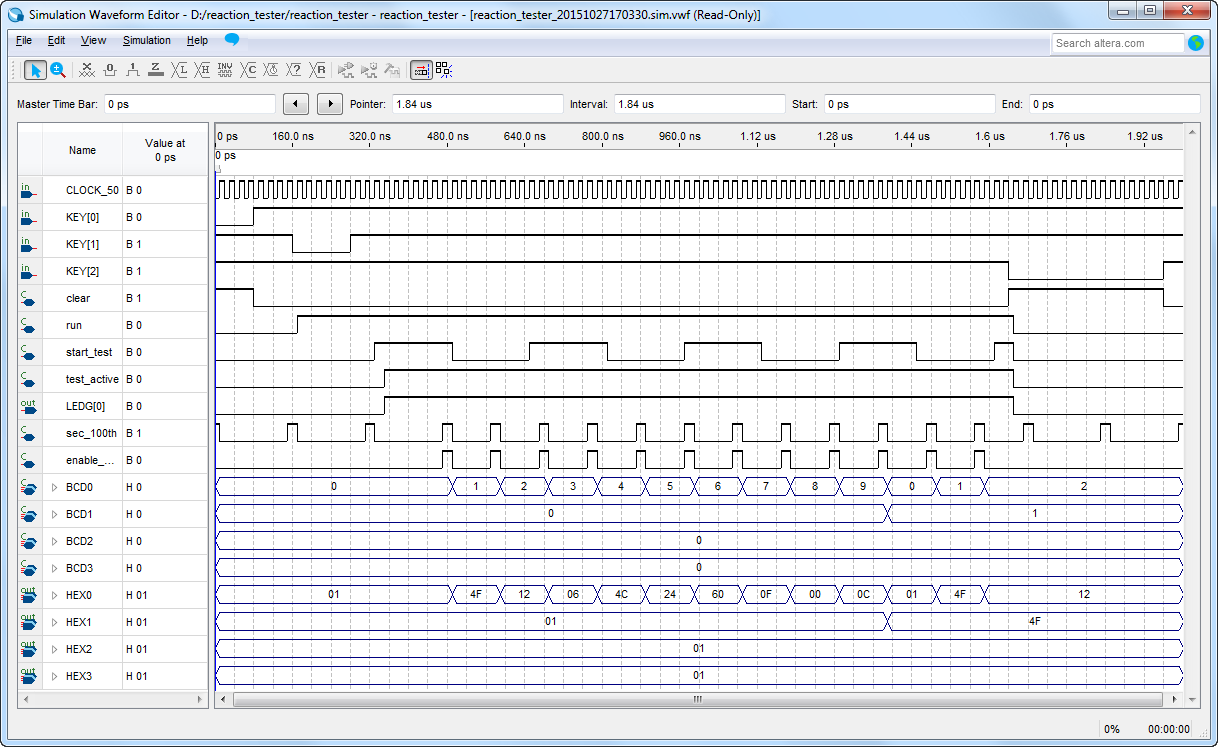
\includegraphics[scale=0.5]{figures/figure20.png}
   \caption{The result of functional simulation.} 
	 \label{fig:20}
	 \end{center}
\end{figure}

Quartus Prime software includes the simulation tools. They are described in
the tutorial {\it Introduction to Simulation of VHDL Designs}.
We encourage the user to use the ModelSim simulator, particularly when large
circuits are involved.

\section{Debugging Concepts}
Debugging of complex logic circuits can be difficult. The task is made easier
if one uses an organized approach with the aid of debugging tools.
The debugging task involves:
\begin{itemize}
\item Observing that there is a problem
\item Identifying the source of the problem
\item Determining the design changes that have to be made
\item Changing and re-implementing the designed circuit 
\item Testing the corrected design
\end{itemize}

\subsection{Observing a Problem}
Often it is easy to see that there is a problem because the designed circuit
does not match the designer's expectations in an obvious way.
For example, a graphical image of the circuit displayed by the RTL Viewer
may indicate that there are missing logic blocks and/or connections.

Consider an error where line 39 in Figure~\ref{fig:2} reads
\begin{center}
\begin{tabular}{c}
\begin{lstlisting}[language=VHDL]
enable_bcd <= test_active;
\end{lstlisting}
\end{tabular} 
\end{center}

\noindent
Compiling the design and testing the resulting circuit would show that the
circuit simply does not work. Examining the designed circuit with the RTL Viewer
gives the image in Figure~\ref{fig:21}. It is apparent that there is no output from
the block {\it hundredth\_sec}. The reason is that the Compiler recognized
that the signal {\it sec\_100th} is not used as an input anywhere in the
rest of the circuit, hence it omitted this signal.
Making this observation the designer would quickly discover the error in line 39.
\begin{figure}[H]
   \begin{center}
      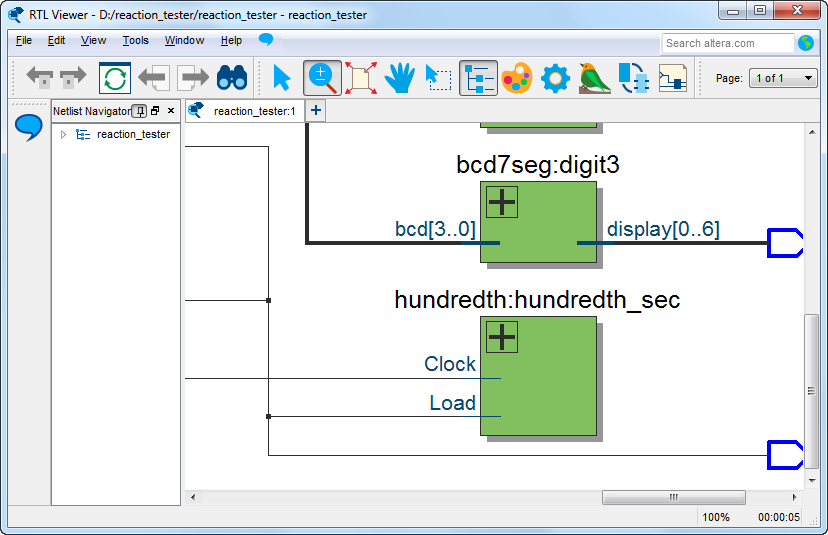
\includegraphics[scale=0.60]{figures/figure21.png}
   \caption{The erroneous circuit displayed by the RTL Viewer.} 
	 \label{fig:21}
	 \end{center}
\end{figure}

As another example, suppose that the designer assumes erroneously that the 
elements of a VHDL vector that refers to the segments of a 7-segment 
display are labeled as going from 6 to 0, which would mean that line 7 in 
Figure~\ref{fig:2} would read 
\begin{center}
\begin{tabular}{c}
\begin{lstlisting}[language=VHDL]
HEX3, HEX2, HEX1, HEX0 : OUT STD_LOGIC_VECTOR(6 DOWNTO 0);
\end{lstlisting}
\end{tabular} 
\end{center}

\noindent
Compiling the design would result in a circuit that seems to respond properly
to pressing of the input keys, but generates a strange-looking output on the
7-segment displays. Observing this behavior, the designer may suspect that there
is something wrong with the display of BCD digits. A possible test is to
see if the BCD counter generates a plausible result, which is easily accomplished
by using the SignalTap Logic Analyzer. Figure~\ref{fig:22} shows an image that we obtained
by triggering on the {\it clear} signal's rising edge (going from 0 to 1), which 
happens in response to {\it KEY}$_2$ being pressed causing the timer to stop counting.
The logic analyzer display indicates that the BCD value should be 0021. However,
the 7-segment displays depict the two least-significant digits as 51 and the two
most-significant digits as upside-down letters AA. The latter fact provides an
immediate clue because the difference between the inverted A and the expected 0
is in segments labeled 0 and 6 in Figure~\ref{fig:12}, which are reversed. This should lead to
a quick detection of the error that we created.

Note also that Figure~\ref{fig:22} indicates that the control signals appear to
work correctly. One clock cycle after the active edge of the {\it clear}
signal, the {\it start\_test} and {\it test\_active} signals go to 0.
The {\it sec\_100th} and {\it enable\_bcd} signals are both equal to 0,
because they are equal to 1 only during one clock cycle in a 1/100 second period.

\begin{figure}[H]
   \begin{center}
      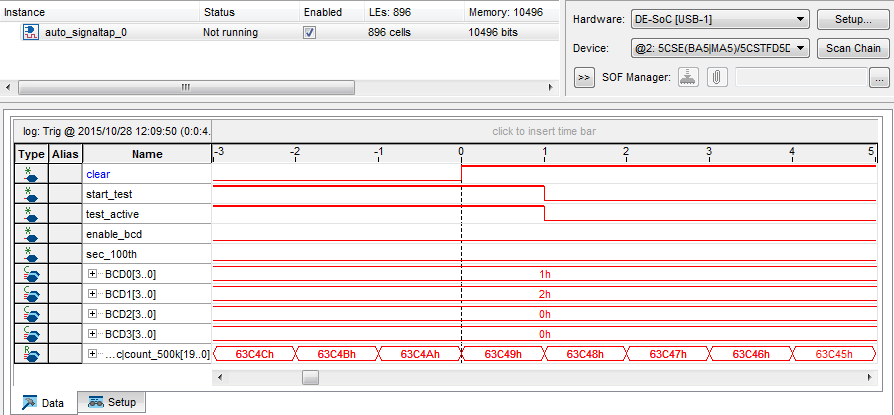
\includegraphics[scale=0.65]{figures/figure22.png}
   \caption{Using the SignalTap Logic Analyzer to observe the output of the BCD counter.} 
	 \label{fig:22}
	 \end{center}
\end{figure}

A complex circuit may be difficult to debug. The circuit implementation may appear 
to contain all necessary components, it may appear to function properly, but the 
results it produces do not exhibit the expected behavior. In such cases, the 
first task is to identify the source of the problem.

\subsection{Identifying the Problem}
Designer's intuition (which improves greatly with experience) may suggest some 
tests that could be tried. Otherwise, it is necessary to adopt an organized
procedure. A golden rule is to first test small portions of the circuit, which
should be easy to do if the circuit is designed in modular fashion. This is
referred to as the divide-and-conquer approach.

Our example circuit is constructed in modular fashion. Each module in Figure~\ref{fig:1}
can be tested separately by using the SignalTap Logic Analyzer. It is 
also useful to compile, simulate and test each module on its own, before it is 
included in the bigger circuit.

It may be helpful to functionally exercise only a portion of a designed circuit, 
which can show whether or not this portion is working correctly. For example,
we can test the BCD counter and the 7-segment displays by isolating this
part from the rest of the circuit and providing separately-controlled inputs
to this subcircuit. One way of doing this is to use a manual clock instead
of the system clock, which would allow us to see the changes (on the 7-segment
displays) that take place during the counting process. To accomplish this,
we can change line 45 in Figure~\ref{fig:2} to read
\begin{center}
\begin{tabular}{c}
\begin{lstlisting}[language=VHDL]
bcdcount: BCD_counter PORT MAP(KEY(2), request_test, '1', BCD3, BCD2, BCD1, BCD0);
\end{lstlisting}
\end{tabular} 
\end{center}
\noindent
Now, {\it KEY}$_2$ is used as a manual clock and the counter is enabled at
all times (by connecting 1 to the enable input). Once these changes have been implemented, pressing {\it KEY}$_2$
repeatedly will step the counter in the upward direction which should be 
observable on the displays. Note that the BCD counter can be cleared by
pressing {\it KEY}$_1$, but only when an active clock signal edge arrives
(as a result of pressing {\it KEY}$_2$) because the {\it BCD\_counter} module
uses synchronous clear.

\section{Sources of Errors in VHDL Designs}
The Quartus Prime Compiler can detect many errors in VHDL files that specify
a given circuit. Typical errors include incorrect syntax, undeclared inputs or 
outputs, improper use of variables and incorrect sizes of vectors.
The compiler stops compilation and displays an error message.
Such errors are usually easy to find and correct. It is much more difficult
to find errors in a circuit that appears to be correctly specified but the
specification does not result in a circuit that the designer hoped to achieve.  
In this section we will consider some typical errors of this type.

Some common errors in VHDL designs are:
\begin{itemize}
\item Inadvertent creation of latches
\item Omission of signals
\item Not assigning a value to a wire
\item Assigning a value to a wire more than once
\item Incorrect specification of PORT MAP signals
\item Wrong definition of a signal vector
\item Incorrectly specified FSM (e.g. wrong or invalid next state)
\item Incorrect timing where the output signal of a given circuit is off
by one clock cycle
\item Careless use of clocks
\end{itemize}

Inadvertent latches are created by the Compiler if the designer fails to
specify the action needed for all cases in constructs where a certain number
of cases are expected to be specified in what is supposed to be a
combinational circuit (e.g. in IF-ELSE and CASE statements). 

If the designer fails to use some signals in a VHDL design file, the
Compiler will ignore these signals completely and may even omit the
circuitry associated with these signals.

Failure to include the BEGIN and END delimiters in a multi-statement
PROCESS block will cause only one statement to be considered valid.

Careful use of blocking and nonblocking assignments is essential. It is
dangerous, and not advisable, to use both types of assignments in the
same PROCESS block. To describe a combinational circuit in a PROCESS
construct, it is best to use blocking assignments. For sequential circuits,
one should use nonblocking assignments.

Incorrect definitions of signal vectors lead to problems, as illustrated in
section 5.1.

Errors in the specification of an FSM may lead to a variety of undesirable
consequences. They can cause wrong functional behavior by reaching wrong states,
as well as wrong timing behavior by producing incorrect output signals.
A common error results in an output signal that is off by one clock cycle.

It is particularly important to use clocks carefully. For example, a slower
clock may be derived by using a counter to divide down the main system clock.
Timing problems may arise when signals generated in a circuit controlled
by one clock are used as inputs to a circuit controlled by a different clock.
Whenever possible, all flip-flops should be driven by the same clock.
For instance, if a given counter has to be incremented/decremented at a rate that 
is slower than the system clock rate, it is best to drive the counter with the 
system clock and use a slower changing {\it enable} signal to make the
counter count at a slower rate. We used this approach in our example circuit
to control the BCD counter.

\section{Errors Due to Wrong Interpretation of Board Characteristics}
Inadequate understanding of the DE-series board can lead to design errors.
Typical examples include:
\begin{itemize}
\item Wrong pin assignment
\item Wrong interpretation of the polarity of pushbutton keys and toggle switches
\item Timing issues when accessing various chips on the board, such as the SDRAM memory
\end{itemize}

If pins are not assigned correctly, the circuit will not exhibit the desired 
behavior. This may be easy to detect when obviously observable input and output signals
are involved. If the designer specifies a wrong assignment for a pushbutton key,
then pressing this key will probably have no effect. If the connection to 
a 7-segment display is not made at all, the display will show the pattern 8.
This means that all seven segments are driven by a logic 0 signal, because a
segment lights up when connected to ground voltage. The Quartus Prime Compiler
causes all unused pins to be driven to ground by default. (Of course, this
default choice can be changed (in the Quartus Prime project) by specifying a 
different option for the unused pins.) The easiest way of ensuring that the pins
are correctly assigned for the DE-series board is to import the pin-assignment file 
for your DE-series board from the FPGA University Program's website.

Pushbutton switches produce logic 0 when pressed. Toggle switches
generate logic 1 when in the up position (towards the middle of the board).

If the design involves access to the SDRAM chip, it is necessary to adhere to
strict timing requirements, as explained in the tutorial
{\it Using the SDRAM Memory on Intel's DE-Series Board with VHDL Designs}.

\section{Design Procedure}
It is prudent to follow a design procedure that tends to minimize the number
of design errors and simplifies the debugging task. Here are some suggestions that 
are likely to help:
\begin{itemize}
\item Design the circuit in a modular, hierarchical manner.
\item Use well-understood and commonly-used constructs to define circuits.
\item Test each module, by simulating it, before it is incorporated into 
the larger circuit.
\item Define and test portions of the final circuit by connecting two or
more modules.
\item Construct the complete circuit and test it through simulation.
Both functional and timing simulation should be done.
\item Download the compiled circuit into the FPGA on the DE-series board and
test it.
\end{itemize}

It is prudent to write VHDL code in a style that allows one to easily
visualize the circuit specified by the code. It is also useful to make 
the code easily understandable for other people.   

% Copyright and Trademark

%\newcommand{\datePublished}{Mar 2022}

\newcommand{\versnum}{21.1} %version number quartus/AMP
\newcommand{\quartusname}{Quartus\textsuperscript{\textregistered} Prime}	
\newcommand{\textBar}{For \quartusname{} \versnum{}}
\newcommand{\thisyear}{2022 } %for copyright
\newcommand{\company}{FPGAcademy.org}
\newcommand{\longteamname}{FPGAcademy.org}
\newcommand{\teamname}{FPGAcademy}
\newcommand{\website}{FPGAcademy.org}

\newcommand{\productAcronym}{AMP}
\newcommand{\productNameShort}{Monitor Program}

\newcommand{\productNameMedTM}{Monitor Program}
\newcommand{\productNameMed}{Monitor Program}

%\newcommand{\headerLogoFilePath}[1]{#1/FPGAcademy.png}



%%%%%%%%%%%%%%%%%%%%%%%%%%%%%%%%%%%%%%%%
%%% FPGAcademy Copyright Information %%%
%%%%%%%%%%%%%%%%%%%%%%%%%%%%%%%%%%%%%%%%

%Always put the copyright on a new page (clear page), with some vertical space from top
\clearpage
\vspace{1in}

\noindent

Copyright {\copyright} FPGAcademy.org. All rights reserved. FPGAcademy and the FPGAcademy logo are trademarks of  FPGAcademy.org.  This document is being provided on an ``as-is'' basis and as an accommodation and therefore all warranties, representations or guarantees of any kind (whether express, implied or statutory) including, without limitation, warranties of merchantability, non-infringement, or fitness for a particular purpose, are specifically disclaimed.

%FPGAcademy assumes no responsibility or liability arising out of the application or use of any information,  product,  or  service  described  herein  except  as  expressly  agreed  to  in  writing  by  FPGAcademy.



**Other names and brands may be claimed as the property of others.




\end{document}
